\section{Antecedentes}
	
	Para esta investigación se buscaron antecedentes de alcance nacional e internacional que ayuden a guiar, sustentar y validar esta investigación.
	
	\textcite{casallas2005desarrollo}, escribieron para la revista Acción Pedagógica de la Universidad de los Andes un artículo titulado \enquote{Desarrollo básico de un Laboratorio Virtual de Control de Procesos basado en Internet}, fue desarrollado conjuntamente entre la UNET y la ULA para ser usado a través de Internet y cuyo objetivo fue desarrollar un laboratorio virtual de control de procesos para la enseñanza a distancia, permitiendo ser utilizado solo por usuarios registrados y en determinados horarios. Aunque la finalidad de la investigación acá propuesta difiere del objetivo de \citeauthor{casallas2005desarrollo}, esta servirá como ayuda para determinar las funciones más utilizadas en el área de control, así como las necesidades típicas de un laboratorio de control virtual.
	
	Adicionalmente, \textcite{salazar2019diseno}, realizó en la Universidad Técnica del Norte, Ecuador, una tesis titulada \enquote{Diseño de un sistema de riego inteligente para cultivos de hortalizas basado en Fuzzy Logic en la granja la pradera de la Universidad Técnica del Norte.} para la implementación del controlador basado en la lógica difusa utilizó, entre otros equipos, un Rasberry PI para la ejecución de Python, específicamente, hizo uso de la biblioteca Scikit-Fuzzy, la cual le permitió definir las funciones de membresía, establecer las reglas difusas, realizar los procesos de fuzzificación y defuzzificación, todo lo mencionado sera para una arquitectura de controlador difuso tipo Mamdani. Esta tesis servirá como referencia para establecer el diseño de controladores difusos utilizando la biblioteca Scikit-Fuzzy.

	Por otro lado, \textcite{congo2018aplicaciones} realizó en la Universidad Tecnológica Israel, Ecuador, una tesis titulada \enquote{Aplicaciones del software libre Python para prácticas de laboratorio aplicado a la asignatura de tratamiento digital de señales de la Universidad Tecnológica Israel} cuyo objetivo fue desarrollar por medio del software Python y sus diferentes librerías científicas, la realización de 3 Prácticas de Laboratorio para la asignatura Procesamiento Digital de Señales de la Universidad Tecnológica Israel, al igual que la intención de este trabajo, se realizó una interfaz gráfica con el objetivo de facilitar su uso, en este caso como herramienta para el procesamiento digital de señales. Este trabajo sustenta la viabilidad de realizar una interfaz gráfica con enfoque similar en el campo de la electrónica y se utilizará como guía parcial para establecer su uso en sistemas de control.
	
	Finalmente, \textcite{cadavid2009toolbox} redactó para la revista Educación en Ingeniería de Colombia, un artículo titulado \enquote{Toolbox didáctico para el diseño y análisis de sistemas de control lineal}, cuyo objetivo es describir un toolbox realizado en MATLAB para el análisis de sistemas de control lineales, este toolbox consiste de una interfaz gráfica que permite realizar pruebas a sistemas de control como respuesta escalón, respuesta en frecuencia, análisis de estabilidad, diseño de controladores, entre otras funciones. Este artículo será de utilidad para establecer la interfaz gráfica que se pretende realizar, además, sirvió como punto de partida para determinar las funciones que debería tener un laboratorio virtual de sistemas de control, como punto adicional se puede resaltar que reafirma la utilidad de esta investigación. 
	
\section{Bases teóricas}
	
    Para poder realizar el laboratorio virtual de sistemas de control clásicos y difusos será necesario abarcar conocimientos de análisis de sistemas de control, diseño de controladores PID y controladores difusos, a continuación, se presentan los conceptos necesarios para el desarrollo de esta investigación.
    
    \subsection{Procesos}
		
		Es importante partir de la base, es por ellos que empezaremos con los procesos, \textcite{sanchez2003control} define los procesos como \enquote{[...] un bloque que se identifica porque tiene una o más variables de salida de las cuales es importante conocer y mantener sus valores}(p.$\,$153). Así, un proceso se caracteriza por tener una entrada y una salida (para procesos SISO), dicha salida deberá mantenerse alrededor de un punto de referencia dado, es decir, se debe controlar su salida.
	
	\subsection{Modelado de procesos en tiempo continuo}
	
		Un proceso puede ser representado por ecuaciones diferenciales que determinen su comportamiento dinámico en el dominio del tiempo, no obstante, trabajar con ecuaciones diferenciales es tedioso a nivel matemático, por tanto, se prefiere modelar los procesos utilizando la transformada de Laplace para llevar de una representación dinámica a una algebraica. Esta ecuación algebraica se operará para llevar a una función de transferencia que represente al proceso en el dominio de la frecuencia compleja \Parencite{smith1985principles}.
	
		\subsubsection{Transformada de Laplace}
		
			La transformada de Laplace de una función dependiente del tiempo f(t) viene dada por la ecuación:
			
			\begin{equation}\label{eq:Laplace}
				F(s) = \mathcal{L}\left[f(t) \right] = \int_{0}^{\infty} f(t)e^{-st}dt
			\end{equation}
			
			\noindent si suponemos que f(t) es un proceso cuya representación dinámica viene dada por una ecuación diferencial de la forma:
			
			\begin{equation}\label{eq:Diffeq}
				a_{2}\frac{d^{2}y(t)}{dt^{2}} + a_{1}\frac{dy(t)}{dt} + a_{0}y(t) = b_{0}x(t)
			\end{equation}
			
			Aplicando \cref{eq:Laplace} a \cref{eq:Diffeq}  y despejando la relación $Y(s)/X(s)$ para el proceso con condiciones iniciales igual a cero (debido a que el proceso debe ser lineal) se obtiene la correspondiente función de transferencia del proceso $H(S)$:
			
			 \begin{equation}\label{eq:TransferFunction}
			 	H(s) =	\frac{Y(s)}{X(s)} = \frac{b_{0}}{a_{2}s^{2} + a_{1}s + a_{0}}
			 \end{equation}
			 
			 La demostración completa \Parencite[pp.$\,$21-22]{smith1985principles} no es de interés para este trabajo, pero si su resultado, la función de transferencia puede ser analizada para determinar las características del proceso, como su ganancia, constante de tiempo, tiempo muerto, entre otras.
			 
		 \subsubsection{Ecuaciones de espacio de estado}
		 
		 	Las ecuaciones de espacio de estado son un método más moderno para modelar todo tipo de sistemas, no solo físicos, sino también biológicos, económicos, sociales y otros. Así como una ecuación diferencial puede ser representada como una función de transferencia también se puede representar como una ecuación de espacio de estados, por tanto, una función de transferencia también puede ser representada en el espacio de estados y viceversa. Las ecuaciones linealizadas alrededor de un estado de operación \Parencite[p.$\,$31]{ogata2003ingenieria} son:
		 
			\begin{align}
                \dot{x}(t) &= Ax(t) + Bu(t) \label{eq:SSrepresentationX} \\
				y(t) &= Cx(t) + Du(t) \label{eq:SSrepresentationY}
			\end{align}
			
			\begin{spacing}{1.5}
				\noindent con: 
				
				$A$: como matriz de estado.
				
				$B$: como matriz de entrada.
				
				$C$: como matriz de salida.
				
				$D$: como matriz de transmisión directa.
				
            \end{spacing}
            
            Normalmente la notación presentada en las ecuaciones \cref{eq:SSrepresentationX,eq:SSrepresentationY} es preferida dado que son compactas y fáciles de entender, no obstante, es al expandir las ecuaciones en su forma matricial que podemos ver claramente que la ecuación \cref{eq:SSrepresentationX} es un sistema de ecuaciones diferenciales ordinarias:
            
            \vspace{20pt}
            \begin{align}
                \begin{bmatrix}
                    \dot{x}_{1}\\
                    \dot{x}_{2}\\
                    \vdots\\
                    \dot{x}_{n}\\
                    \end{bmatrix}&=
                    \begin{bmatrix}
                    a_{11} & a_{12} & \cdots & a_{1n}\\
                    a_{21} & a_{22} & \cdots & a_{2n}\\
                    \vdots & \vdots & \ddots & \vdots\\
                    a_{n1} & a_{n2} & \cdots & a_{nn}\\
                    \end{bmatrix}
                    \begin{bmatrix}
                    x_{1}\\
                    x_{2}\\
                    \vdots\\
                    x_{n}\\
                    \end{bmatrix}+
                    \begin{bmatrix}
                    b_{11} & b_{12} & \cdots & b_{1m}\\
                    b_{21} & b_{22} & \cdots & b_{2m}\\
                    \vdots & \vdots & \ddots & \vdots\\
                    b_{n1} & b_{n2} & \cdots & b_{nm}\\
                    \end{bmatrix}.
                    \begin{bmatrix}
                    u_{1}\\
                    u_{2}\\
                    \vdots\\
                    u_{m}\\
                    \end{bmatrix}\label{eq:FullSSx}\\
                    \begin{bmatrix}
                    y_{1}\\
                    y_{2}\\
                    \vdots\\
                    y_{n}\\
                    \end{bmatrix}&=
                    \begin{bmatrix}
                    c_{11} & c_{12} & \cdots & c_{1n}\\
                    c_{21} & c_{22} & \cdots & c_{2n}\\
                    \vdots & \vdots & \ddots & \vdots\\
                    c_{r1} & c_{r2} & \cdots & c_{rn}\\
                    \end{bmatrix}
                    \begin{bmatrix}
                    x_{1}\\
                    x_{2}\\
                    \vdots\\
                    x_{n}\\
                    \end{bmatrix}+
                    \begin{bmatrix}
                    d_{11} & d_{12} & \cdots & d_{1m}\\
                    d_{21} & d_{22} & \cdots & d_{2m}\\
                    \vdots & \vdots & \ddots & \vdots\\
                    d_{r1} & d_{r2} & \cdots & d_{rm}\\
                    \end{bmatrix}.
                    \begin{bmatrix}
                    u_{1}\\
                    u_{2}\\
                    \vdots\\
                    u_{m}\\
                    \end{bmatrix}
            \end{align}
            \vspace{20pt}

            \begin{spacing}{1.5}
				\noindent con: 
				
				$n$: como el numero de variables de estado
				
				$m$: como el numero de entradas
				
				$r$: como el numero de salidas
				
            \end{spacing}

            Para resolver sistemas de ecuaciones diferenciales podemos utilizar métodos iterativos como los de Runge-Kuuta.

    \subsection{Modelado de procesos en tiempo discreto}

        Así como para tiempo continuo se utilizan ecuaciones diferenciales, en el tiempo discreto se hace uso de ecuaciones en diferencias. Las ecuaciones en diferencias se pueden utilizar para aproximar a las ecuaciones diferenciales, estas primeras se suelen utilizar porque son más fáciles de programar \Parencite{kuo1996sistemas}, por lo cual los procesos pueden ser representados de la siguiente forma:
        
        \begin{equation}\label{eq:EqEnDiferencias}
            y(k+n) + a_{n-1}y(k+n-1) + \cdots + a_1 y(k+1) + a_0 y(k) = f(k) 
        \end{equation}
        
        Asi mismo debido a que la ecuacion \cref{eq:SSrepresentationX} esta compuesta de ecuaciones diferenciales, esta puede ser llevada a una ecuacion en diferencias y la representacion del proceso en el espacio de estados queda como sigue:

        \begin{align}\label{eq:SSdiscreto}
            x(k+1) &= A_d x(k) + B_d u(k) \\
            y(k) &= C_d x(k) + D_d u(k)
        \end{align}

        \subsubsection{Transformada z}
		
			En tiempo discreto se puede modelar un proceso utilizando la transformada z sobre la ecuación en diferencias del proceso para obtener su representacion en el dominio Z, la transformada Z es a las ecuaciones en diferencia lo que la transformada de laplace es las ecuaciones en tiempo continuo, la ecuación general para la transformada z es:
			
			\begin{equation}\label{eq:Ztransform}
				F(z)= \sum\limits_{k=0}^{\infty}f(k)z^{-k}
			\end{equation}

        \subsubsection{Discretizacion de una funcion de transferencia continua}
            
            Existen varios metodos para realizar la discretizacion de una funcion de transferencia continua, el metodo mas simple suele implicar el uso de un muestreador con un retensor de orden zero (ZOH), retensor de orden zero significa que la señal de entrada es retenida constantemente durante el intervalo de muestreo \Parencite{haugen2005discrete}, la formula para realizar la discretizacion con retensor de orden zero es la siguiente:

            \begin{equation}\label{eq:ZOH}
                H(z) = (1 - z^{-1}) \mathcal{Z} \left[ \mathcal{L}^{-1}\left\lbrace \frac{G(s)}{s}\right\rbrace\Bigr|_{t=kh}\right]
            \end{equation}

            Existen otros modos de llevar una función de transferencia continua al dominio Z como las aproximaciones de Tustin y Euler, estas consisten en sustituir la variable s por una aproximación en el dominio Z y se sustentan en ser aproximaciones numéricas a integrales en el tiempo, \textcite{haugen2005discrete} afirma que la aproximacion de Tustin es la mas precisa de las tres, no obstante, sugiere que no existe una diferencia notable entre este y Euler hacia atrás, ademas, la mayoría de los controladores comerciales vienen con Euler hacia atrás, por lo que puede considerarse una mejor opción a la hora de escoger un método. Las sustituciones correspondientes son:

            \begin{align}
                &\text{Euler hacia adelante:}& &s \leftarrow \frac{z - 1}{h} \label{eq:eulerF}\\
                &\text{Euler hacia atrás:}& &s \leftarrow \frac{z - 1}{hz} \label{eq:eulerB}\\
                &\text{Tustin:}& &s \leftarrow \frac{2}{h} \frac{z-1}{z+1} \label{eq:tustin}
            \end{align}
    
    \subsection{Respuesta en el tiempo del modelo en el espacio de estados}
        
        Para poder obtener la respuesta del sistema en el tiempo podemos utilizar varios metodos de resolucion de ODE's o ecuaciones diferenciales ordinarias, solucion exacta, separacion de variables o integracion numerica aproximada, este ultimo es el mejor para realizar por medio de computadoras. Para realizar la integracion numerica y obtener la respuesta del sistema se utilizaran los metodos de Runge-Kutta.

        Los metodos de Runge-Kutta son unos metodos iterativos de resolución de ODE's, los mismos se basan en utilizar \blockquote[{\cite[p.31]{horacio1997metodos}}]{indirectamente el algoritmo de Taylor. En general, estos metodos evalúan $f(x,y)$ en mas de un punto en la proximida $(x_n,y_n)$ en lugar de evaluar derivadas de $f(x,y)$}. La formulación general de los metodos de Runge-Kutta explícitos es:
        
        \begin{equation}\label{eq:RKgeneral}
            \begin{aligned}
                k_1 &= f(x_0,y_0)\\
                k_2 &= f(x_0 + c_2 h,y_0 + ha_{21}k_1)\\
                k_3 &= f(x_0 + c_3 h,y_0 + h(a_{31}k_1 + a_{32}k_2))\\
                &\mathrel{\makebox[\widthof{=}]{\vdots}}\\
                k_s &= f(x_0 + c_s h,y_0 + h(a_{s1}k1 + \cdots +  a_{s,s-1}k_{s-1}))\\
                y_1 &= y_0 + h(b_1 k_1 + \cdots + b_s k_s)
            \end{aligned}
        \end{equation}
        
        Donde $s$ denota el numero de escenarios a utilizar, es comun expresar \cref{eq:RKgeneral} utilizando una tabla de butcher, en honor a John C. Butcher y su articulo de 1964b, por tanto, \cref{eq:RKgeneral} puede representarse de la siguiente forma:

        \begin{equation}\label{eq:explicitoButcher}
            \renewcommand\arraystretch{1.2}
            \begin{array}
            {c|ccccc}
            0\\
            c_2 & a_{21}\\
            c_3 & a_{31} & a_{32}\\
            \vdots & \vdots & \vdots & \ddots\\
            c_s & a_{s1} & a_{s2} & \cdots & a_{s,s-1}\\
            \hline
            & b_1 & b_2 & \cdots & b_{s-1} &  b_{s}
            \end{array}
        \end{equation}

        Adicionalmente existen los metodos de Runge-Kutta embebidos, los cuales consisten en calcular dos metodos de orden $p$ y orden $\hat{p}$ respectivamente, donde $\hat{p}$ es normalmente $p-1$ o $p+1$ \Parencite{hairer1991solving}. La tabla de butcher para representar los metodos embebidos es la siguiente:

        \begin{equation}\label{eq:embebidoButcher}
            \renewcommand\arraystretch{1.2}
            \begin{array}
            {c|ccccc}
            0\\
            c_2 & a_{21}\\
            c_3 & a_{31} & a_{32}\\
            \vdots & \vdots & \vdots & \ddots\\
            c_s & a_{s1} & a_{s2} & \cdots & a_{s,s-1}\\
            \hline
            & b_1 & b_2 & \cdots & b_{s-1} &  b_{s}\\
            \hline
            & \hat{b}_1 & \hat{b}_2 & \cdots & \hat{b}_{s-1} &  \hat{b}_{s}
            \end{array}
        \end{equation}

        \begin{align}
            y_1 &= y_0 + h(b_1 k_1 + \cdots + b_s k_s) & &\text{Orden $p$}\\
            \hat{y}_1 &= y_0 + h(\hat{b}_1 k_1 + \cdots +\hat{b}_s k_s) & &\text{Orden $\hat{p} = p-1$ o $p+1$}
        \end{align}

        De modo que la integración para el siguiente paso se continua con $y_1$, el fin de calcular dos metodos en conjunto es para poder estimar el error y poder realizar un cambio en el tamaño de paso, de este modo, se puede incrementar el tamaño de paso si el error es muy bajo o disminuirlo si el error es inaceptable.
        
        \subsubsection{Runge-Kutta's para ecuaciones de espacio de estados}

            Partiendo de la ecuación \cref{eq:FullSSx} en donde podemos observar que $\dot{x}(t)$ viene dado por un conjunto de ecuaciones diferenciales ordinarias, por tanto, es posible aplicar los metodos de Runge-Kutta de forma casi directa, \textcite{horacio1997metodos} desarrolla las expresiones para un Runge-Kutta de orden 4 aplicado en el espacio de estados, estas expresiones pueden ser extendidas para generalizar su aplicación a un numero de escenarios arbitrarios, el vector de estados de forma general se puede expresar como:

            
            \begin{equation}\label{eq:vectorGeneral}
                \begin{aligned}
                    x_1(t) &= f_1(t, x_1, x_2, \dots, x_n) = f_1(t,x)\\
                    &\mathrel{\makebox[\widthof{=}]{\vdots}}\\
                    x_n(t) &=  f_n(t,x)
                \end{aligned}
            \end{equation}

            \noindent cuyas condiciones iniciales se pueden expresar como:

            \begin{equation}\label{eq:vectorIniciales}
                \begin{aligned}
                    x_1^{(0)} &= \alpha_1\\
                    &\mathrel{\makebox[\widthof{=}]{\vdots}}\\
                    x_n^{(0)} &=  \alpha_n
                \end{aligned}
            \end{equation}
            
            \noindent de modo que al sustituir \cref{eq:vectorGeneral,eq:vectorIniciales} en \cref{eq:RKgeneral} y señalando:

            \vfill 

            \begin{spacing}{1.5}
				
				$n$: como el numero de variables de estado
				
				$m$: como el numero de entradas
				
				$j$: como la iteración actual
                
                $s$: como el numero de escenarios
            \end{spacing}

            \vfill
            \pagebreak

            \noindent se obtenga el nuevo vector de estado:

            \begin{equation}\label{eq:RKstate}
                \begin{aligned}
                    k_1 &= Ax_n^{(j)} + Bu_m^{(j)}\\
                    k_2 &= A(x_n^{(j)} +  ha_{21}k_1) + Bu_m^{(j)}\\
                    k_3 &= A(x_n^{(j)} +  h(a_{31}k_1 + a_{32}k_2)) + Bu_m^{(j)}\\
                    &\mathrel{\makebox[\widthof{=}]{\vdots}}\\
                    k_s &= A(x_n^{(j)} + h(a_{s1}k1 + \cdots +  a_{s,s-1}k_{s-1})) + Bu_m^{(j)}\\
                    x_n^{(j+1)} &= x_n^{(j)} + h(b_1 k_1 + \cdots + b_s k_s)
                \end{aligned}
            \end{equation}
            
            \noindent finalmente, el vector de estado obtenido con \cref{eq:RKstate} sera sustituido en la siguiente iteraciones, para obtener la salida actual se debe sustituir $x_n^{(j)}$  en \cref{eq:SSrepresentationY}. 
            
            \begin{equation}
				y^{(j)} = Cx_n^{(j)} + Du_m^{(j)} \label{eq:SSrepresentationY}
            \end{equation}
            
            Los pasos mencionados se repiten una y otra vez de forma iterativa utilizando un tamaño de paso adecuado, el tamaño de paso determinara el numero de iteraciones a realizar, un tamaño de paso pequeño genera resultados mas precisos pero incrementa el tiempo de computo considerablemente, por otro lado, un tamaño de paso grande puede generar errores inaceptables con la ventaja de acelerar los cálculos, el tamaño de paso es un factor muy importante en los metodos de Runge-Kutta.

        \subsubsection{Tamaño de paso variable}

            Como ya se menciono antes, se puede realizar una adaptación del tamaño de paso en función del error y es posible no solo para los metodos embebidos, sino también para los explícitos, \textcite{roganprogramacion} afirma que: \blockquote[p.251]{Los programas adaptativos continuamente monitorean la solución y modifican el paso de
            tiempo para asegurar que se mantenga la precisión especificada por el usuario. Esos programas
            pueden hacer algunos cálculos extras para optimizar la elección de $\tau$ , en muchos casos este
            trabajo extra vale la pena.}
            
            \paragraph{Calculo del error con dos medios pasos}

                Este es un método simple pero eficaz de calcular el error, consiste en realizar un paso simple de tamaño h y comparar su respuesta con la respuesta dada por el mismo método al realizar dos pasos de tamaño $\frac{h}{2}$, de este modo el error $\Delta e$ se puede calcular como la diferencia en valor absoluto de ambas respuestas, $\left|y_{1,h} - y_{2,\frac{h}{2}}\right|$ donde $y_{2,\frac{h}{2}}$ es la salida luego de dos medios pasos.
            
            \paragraph{Calculo del error para metodos embebidos} 

                Los metodos embebidos están hechos para poder realizar este calculo del error, por tanto, no hay que realizar ningún calculo extra y el error puede ser calculado de forma directa como $\Delta e = \left| y_1 - \hat{y}_1\right|$

            \paragraph{Nuevo tamaño de paso}

                Combinando las formulas y algoritmos descritos por \textcite{roganprogramacion}, \textcite{hairer1991solving} y \textcite{ritschel2013numerical} se pueden obtener las formulas para el manejo del error con fines de calcular un nuevo tamaño de paso, lo primero es calcular una escala, este es el único paso que se diferencia entre el método de dos medios pasos y el los metodos embebidos. Para dos medios pasos la escala es:

                \begin{equation}\label{eq:escalaDos}
                    escala = atol + rtol \cdot \frac{\left|y_{1,h}\right| + \left|y_{2,\frac{h}{2}}\right|}{2}
                \end{equation}

                \noindent para los metodos embebidos:

                \begin{equation}\label{eq:escalaEmbebidos}
                    escala = atol + rtol \cdot max(\left| y_1\right|,\left| y_0\right|)
                \end{equation}
        
                A partir de aca las formulas son comunes para ambos metodos. Para continuar, se debe realizar el calculo de un error normalizado, por lo cual se calcula la norma RMS del error dividido por la escala calculada:

                \begin{equation}\label{eq:ErrorNormalizado}
                    ||\Delta e|| = \sqrt{\frac{1}{n} \sum_{i=1}^{n} \left(\frac{\Delta e_i}{escala_i}\right)^2}
                \end{equation}

                \noindent donde i denota el numero de elementos que componen la respuesta, finalmente, el nuevo tamaño de paso viene dado por:
                
                \begin{equation}
                    \left\{
                    \begin{aligned}
                        h_{t+1} &= h_{t}\cdot maxStepIncrease &\quad &Si \quad ||\Delta e|| = 0\\
                        h_{t+1} &= h_{t}\cdot sf_1 \cdot ||\Delta e||^{\frac{-1}{q+1}}  &\quad &Si \quad ||\Delta e|| \leq 1 \\
                        h_{t} &= h_{t}\cdot sf_1 \cdot ||\Delta e||^{\frac{-1}{q+1}}  &\quad &Si \quad ||\Delta e|| > 1 \ ,\ \text{Se descarta la salida}
                    \end{aligned}\right.
                \end{equation}
                
                \noindent con $sf_1$ como un factor de seguridad que evita que el nuevo tamaño de paso para un $||\Delta e||$ dado se repita indefinidamente, y $q$ como el orden del metodo utilizado, en el caso de los Runge-Kutta embebidos, $q$ viene dado por el metodo de menor orden entre $y_1$ y $\hat{y}_1$, notese que si el error se encuentra por arriba de uno, la salida es descartada y se repite el calculo con un nuevo tamaño de paso, el proceso se repite hasta que el error sea igual o menor que uno.
    
    \subsection{Respuesta en el tiempo del modelo en el espacio de estados discreto}
        
        El calculo de la respuesta en el tiempo para el modelo en el espacio de estados discreto es mucho mas simple, no se requiere ningún método de integración aproximado, lo cual se debe a que el calculo puede ser realizado se forma directa   ya que la formula es el algoritmo a seguir \Parencite{haugen2005discrete}. Tomando en consideración la ecuación \cref{eq:SSdiscreto}, basta con sustituir el vector de estado para obtener a $x(k+1)$ y la salida $y(k)$
    
    \subsection{Sistemas de control}
		
		\subsubsection{Sistema en lazo abierto}
		
            Un sistema en lazo abierto es aquel cuya salida no es medida en ningún momento en orden de ajustar la entrada, por lo cual provoca que \enquote{las perturbaciones que se presentan en el proceso ocasionen que sus efectos se sientan en la salida del proceso, es decir, en el valor de la variable controlada}\Parencite[p.$\,$350]{maloney2006electronica}. La mayoría de los sistemas en lazo abierto son estables, pero carecen de utilidad practica al no poder mantenerlos en un punto de referencia debido a las perturbaciones.
            
            Por otro lado, es importante analisar el comportamiento del sistema en lazo abierto para determinar su comportamiento en lazo cerrado, ademas, nos permite determinar sus caracteristicas con el fin de realizar un modelo matematico aproximado del sistema, este es util para realizar la entonacion de los controladores sin tener que trabajar de forma directa con el proceso, el cual puede ser peligroso o inaccesible. La representacion en diagrama de bloques de un sistema en lazo abierto se puede observar en la \cref{fig:esquemaLazoAbierto}.
            
            \begin{figure}[htb]
				\centering
				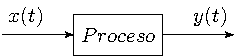
\includegraphics[width=0.5\textwidth]{esquemaLazoAbierto.pdf}
				\caption[Ejemplo de un sistema en lazo abierto]{\textbf{Sistema en lazo abierto}. Fuente: Elaboración propia.} 
				\label{fig:esquemaLazoAbierto}
            \end{figure}
        
        \subsubsection{Sistema en lazo cerrado}
		
			Los sistemas de lazo cerrado son aquellos cuya salida es realimentada a la entrada del sistema, esta realimentación suele ser negativa para que sea estable, no obstante, existen sistemas que se vuelven inestables con el simple hecho de cerrar el lazo, un ejemplo de sistema realimentado se puede observar en la \cref{fig:esquemaLazoCerrado}.
			
			\begin{figure}[htb]
				\centering
				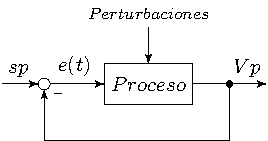
\includegraphics[width=0.6\textwidth]{esquemaLazoCerrado.pdf}
				\caption[Ejemplo de un sistema en lazo cerrado]{\textbf{Sistema en lazo cerrado}. Se observan las principales señales de un sistema en lazo cerrado. Fuente: Elaboración propia.} 
				\label{fig:esquemaLazoCerrado}
			\end{figure}
			
            En la \cref{fig:esquemaLazoCerrado} se denotan algunas de las señales que componen a un sistema de control, $sp$, que corresponde al set point o valor de referencia, $Vp$, que corresponde a la variable del proceso y es la variable a controlar, las perturbaciones, las cuales son magnitudes físicas que pueden afectar al proceso como la temperatura ambiente, presión, vibraciones, entre otras, y finalmente, $e(t)$, que corresponde a la señal de error la cual viene dada por la diferencia entre el valor de referencia y la variable medida \Parencite{maloney2006electronica}.
            
            \begin{equation}\label{eq:Serror}
				e(t) = sp - Vp
            \end{equation}
            
        \subsubsection{Estabilidad de los sistemas}

            La estabilidad se ve afectada por la estructura del sistema, por tanto, se debe tomar en cuanta cuando se cierra el lazo del sistema. \textcite{ogata2003ingenieria} afirma que, desde el punto de vista de estabilidad, el sistema de control en lazo abierto no es un problema importante. Por otra parte, la estabilidad es un gran problema en el sistema de control en lazo cerrado debido a la posibilidad de que se generen oscilaciones. En consecuencia, los análisis de estabilidad se realizan para sistemas en lazo cerrado, el motivo principal es porque los sistemas en lazo abierto tienden a ser estables, además, para realizar el control de un proceso se suele utilizar los sistemas en lazo cerrado

            \paragraph{Análisis de estabilidad en el plano complejo}
            
                La estabilidad de un sistema lineal viene dada por la ubicación de sus polos a lo largo del plano complejo s, i.e., se puede determinar si un sistema es estable si no posee ninguno polo en el semiplano derecho del plano complejo s incluyendo el eje coordenado $j\omega$ en tiempo continuo \Parencite{ogata2003ingenieria}, en el caso de sistemas discretos, los polos deben encontrarse dentro del circulo unitario, la estabilidad marginal es posible si existen uno o mas polos justo en el circulo unitario, pero no multiples. El cual perimite que el análisis de estabilidad se puede realizar de forma analítica y gráfica. En la \cref{fig:pzmap} se puede observar dos sistemas continuos en lazo abierto, $G_1(s)$ que es estable y $G_2(s)$ que es inestable .

                \begin{figure}[htb]
                    \centering
                    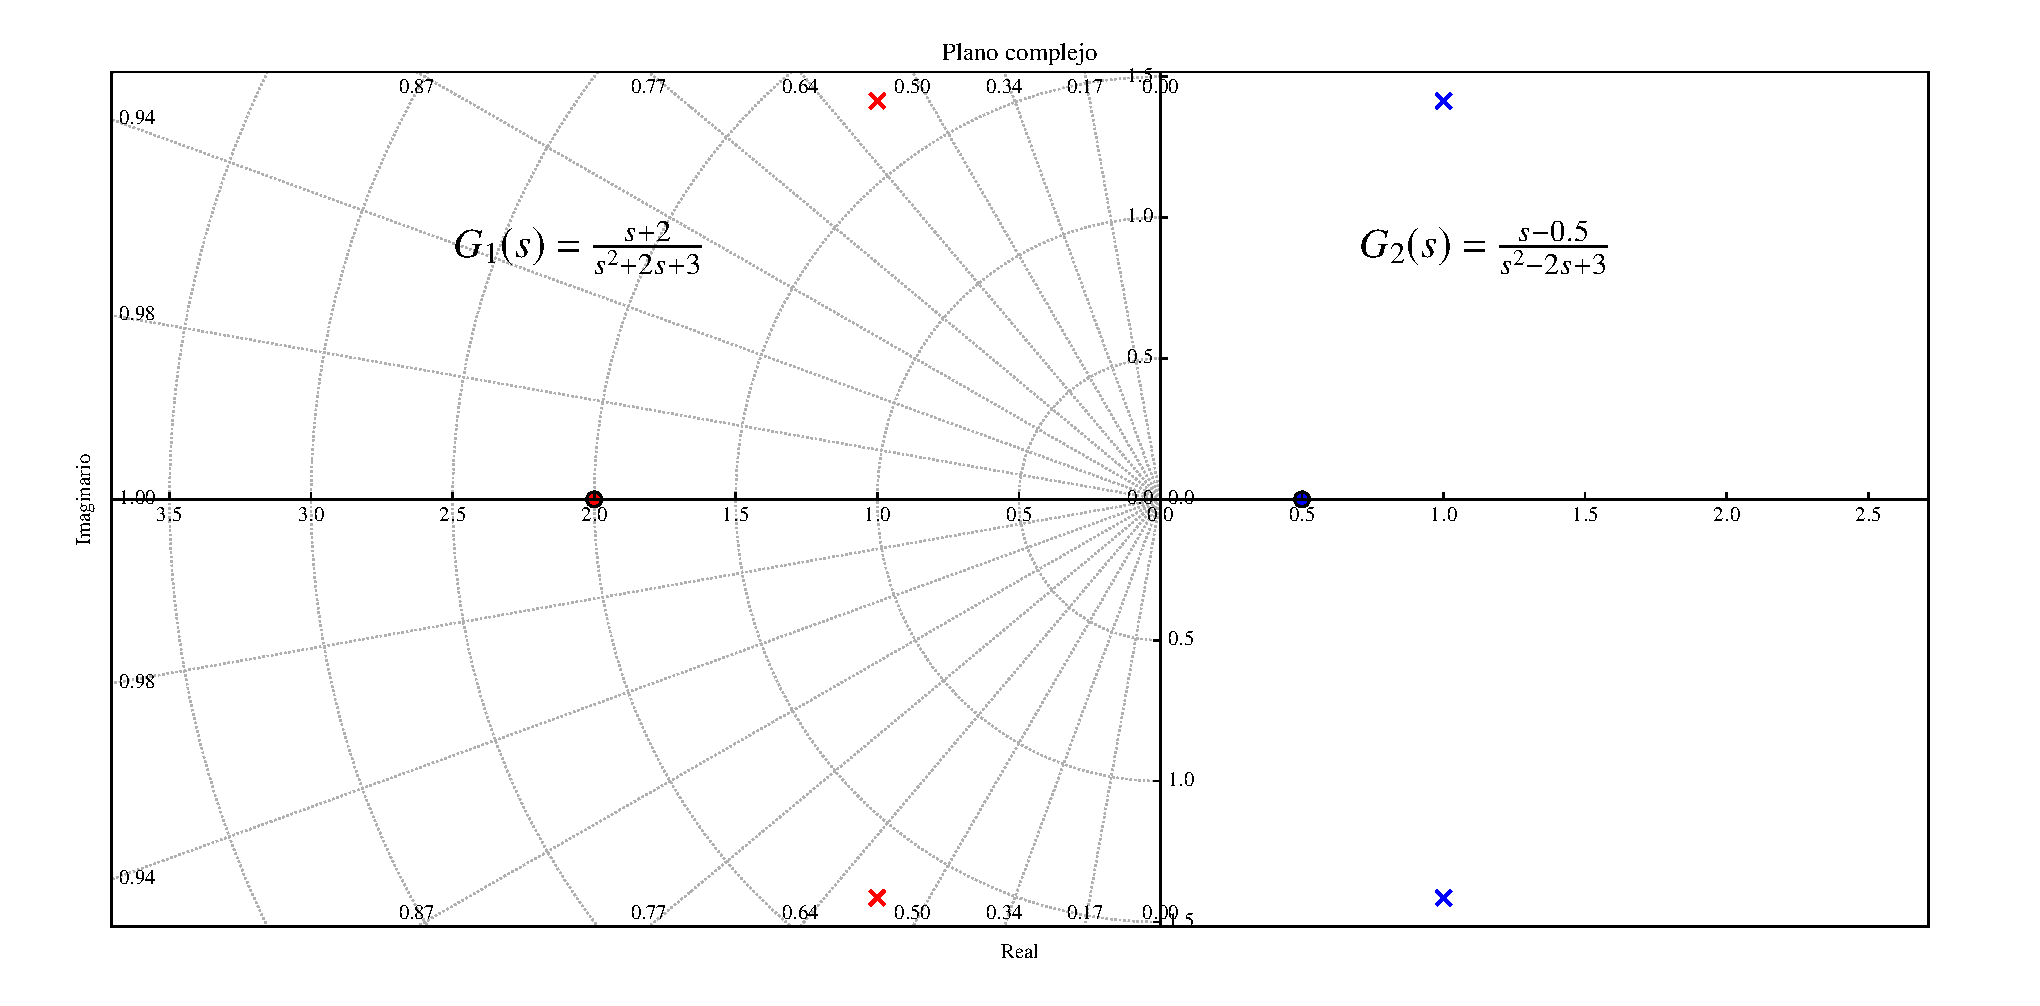
\includegraphics[width=\textwidth]{pzmap.pdf}
                    \caption[Ejemplo de analisis de estabilidad en el plano complejo]{\textbf{Analisis de estabilidad en el plano complejo}. Se puede observar como el sistema $G_1(s)$ tiene ubicado sus polos en el semiplano izquierdo del plano complejo, i.e., es estable, por otro lado, el sistema $G_2(s)$ es inestable al poseer polos ubicados en el semiplano derecho del plano complejo. Fuente: Elaboración propia.} 
                    \label{fig:pzmap}
                \end{figure}
            
            \paragraph{Criterio de estabilidad de Nyquist}
                
                El criterio de estabilidad de Nyquist determina el estado de estabilidad utilizando los polos en lazo abierto y la respuesta en frecuencia del sistema en lazo abierto. Este criterio \enquote{es útil en la ingeniería de control, debido a que permite determinar gráficamente la estabilidad absoluta del sistema en lazo cerrado a partir de las curvas de respuesta en frecuencia en lazo abierto, sin que sea necesario determinar los polos en lazo cerrado}\Parencite[p.$\,$446]{ogata2003ingenieria}. Este criterio tiene la ventaja de poder realizarse tanto con cálculos analíticos como con datos experimentales, \textcite{ogata2003ingenieria} define tres criterios:

                \begin{enumerate}[leftmargin=\parindent]
                    \item El punto $-1 + j0$ no esta rodeado. Esto implica que el sistema es estable en lazo cerrado si no hay polos de $G(s)H(s)$ en el semiplano derecho del plano s\footref{fn:continuevsdiscreto}; de lo contrario, el sistema es inestable.
                    \item El punto $-1 + j0$ queda rodeado una o varias veces en sentido contrario al de las agujas
                    del reloj. En este caso, el sistema es estable en lazo cerrado si el número de rodeos en sentido contrario
                    al de las agujas del reloj es igual al número de polos $G(s)H(s)$ en el semiplano derecho
                    del plano s\footref{fn:continuevsdiscreto}; de lo contrario, el sistema es inestable.

                    \footnotetext[1]{En el caso de sistemas discretos se toma en cuenta son los polos fuera del circulo unitario para la evaluacion de los criterios. \label{fn:continuevsdiscreto}}

                    \item El punto $-1 + j0$ queda rodeado una o varias veces en el sentido de las agujas del reloj.
                    En este caso el sistema es inestable en lazo cerrado.
                \end{enumerate}
                
                En la \cref{fig:nyquistPlot} se puede observar los diagramas de Nyquist para los sistemas presentados en la \cref{fig:pzmap}, el sistema $G_1(s)$ debe ser evaluado por el criterio numero 1, al no poseer ninguno polo en el semiplano derecho el sistema sera estable en lazo cerrado asumiendo un $H(s) = 1$, por otro lado, $G_2(s)$ debe ser evaluado por el criterio numero 2, debido a que el numero de rodeos al punto $-1 + j0$ es igual al numero de polos en el semiplano derecho el sistema sera estable en lazo cerrado asumiendo un $H(s) = 1$ a pesar de que en lazo abierto sea inestable.

                \begin{figure}[htb]
                    \centering
                    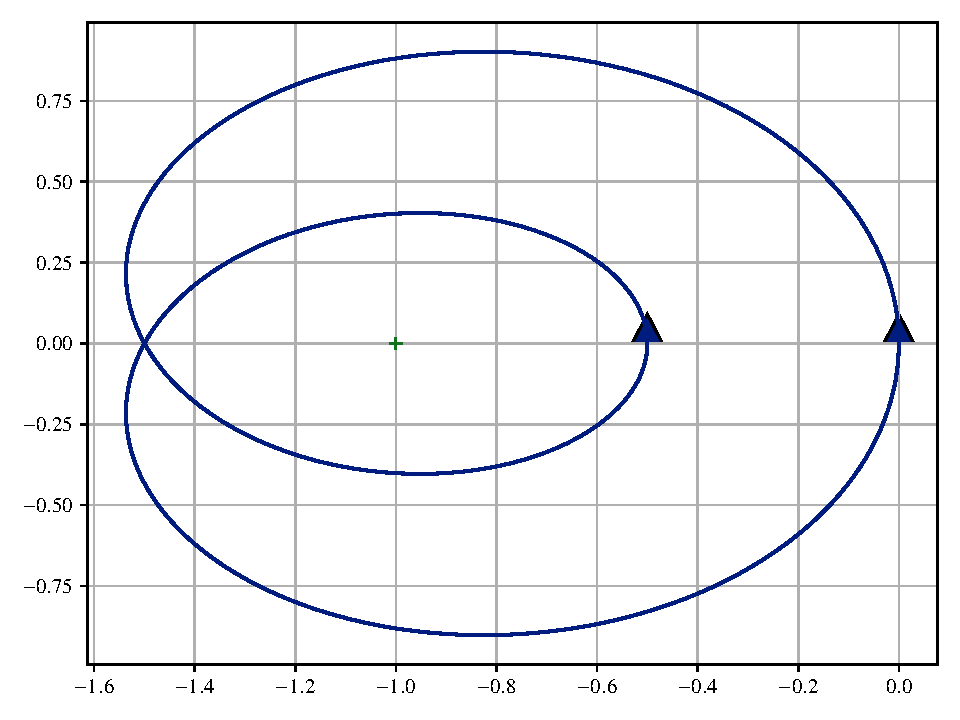
\includegraphics[width=0.7\textwidth]{nyquistPlot.pdf}
                    \caption[Ejemplo de analisis de estabilidad con diagrama de Nyquist]{\textbf{Analisis de estabilidad con diagrama de Nyquist}. El sistema $G_1(s)$ al ser evaluado con el criterio numero 1 se encuentra que es estable en lazo cerrado, a su vez, el sistema $G_2(s)$ al ser evaluado con el criterio numero 2 se encuentra que tambien sera estable en lazo cerrado, en ambos casos se asume un $H(s) = 1$. Fuente: Elaboración propia.} 
                    \label{fig:nyquistPlot}
                \end{figure}
            
            \paragraph{Margen de ganancia y Margen de fase}
                
                Los margenes de ganancia y de fase son una medida de la estabilidad relativa, se toman en cuenta a la hora de realizar el diseño de un controlador debido a que los margenes se pueden interpretar de modo que orienten en la cantidad de ganancia que se le puede aplicar al sistema en lazo cerrado, adicionalmente, la estabilidad relativa se puede interpretar como que tan estable es un sistema. \textcite{dorf2011modern} definen el margen de ganancia como: \blockquote[p.655]{[...] el incremento en la ganancia del sistema cuando $fase = -180^\circ$ que resultaria en un sistema marginalmente estable con la interseccion del punto $-1 + j0$ en el diagrama de Nyquist}. Asi mismo, \textcite{dorf2011modern} definen el margen de fase como: \blockquote[p.656]{[...] la cantidad de desplazamiento de fase de $L(j\omega)$ a una unidad de magnitud que resultaria en un sistema marginalmente estable con la intersección del punto $-1 + j0$ en el diagrama de Nyquist. El margen de ganancia y de fase pueden ser facilmente encontrados utilizando un diagrama de Bode.}

            \paragraph{Análisis de estabilidad con las trazas de Bode}

                Los diagramas de bode son una forma de representar la respuesta en frecuencia de un sistema tomando en cuenta los cambios de amplitud de $L(j\omega)$ y del ángulo de fase de $L(j\omega)$ respecto a la frecuencia \Parencite{nilsson1995circuitos}. Para analizar la estabilidad se utilizan el margen de ganancia y el margen de fase del sistema en un diagrama de Bode a modo de trazas, el punto de estabilidad critica en el diagrama de bode pasa a ser su equivalente en $dB$, el cual es $0dB$.

                Un margen de ganancia positivo y de fase positivos indican que el sistema es estable, si el sistema es de fase no minima, la interpretacion anterior deja de ser valida. Aplicando las deficiones dadas por \textcite{dorf2011modern} podemos obtener el margen de ganancia y de fase para los sistemas $G_1(s)$ y $G_2(s)$ y se presentan como ejemplo en la \cref{fig:bodeG1} y \cref{fig:bodeG2}.

                \begin{itemize}[leftmargin=\parindent]
                    \item $G_1(s)$: $GM \rightarrow \infty$ y $PM \rightarrow \infty$
                    \item $G_2(s)$: $GM = -3.509dB$ a $1.409\ rad/sec$ y $PM = -23.719^\circ$ a $0.807\ rad/sec$
                \end{itemize}

                \begin{figure}[htb]
                    \centering
                    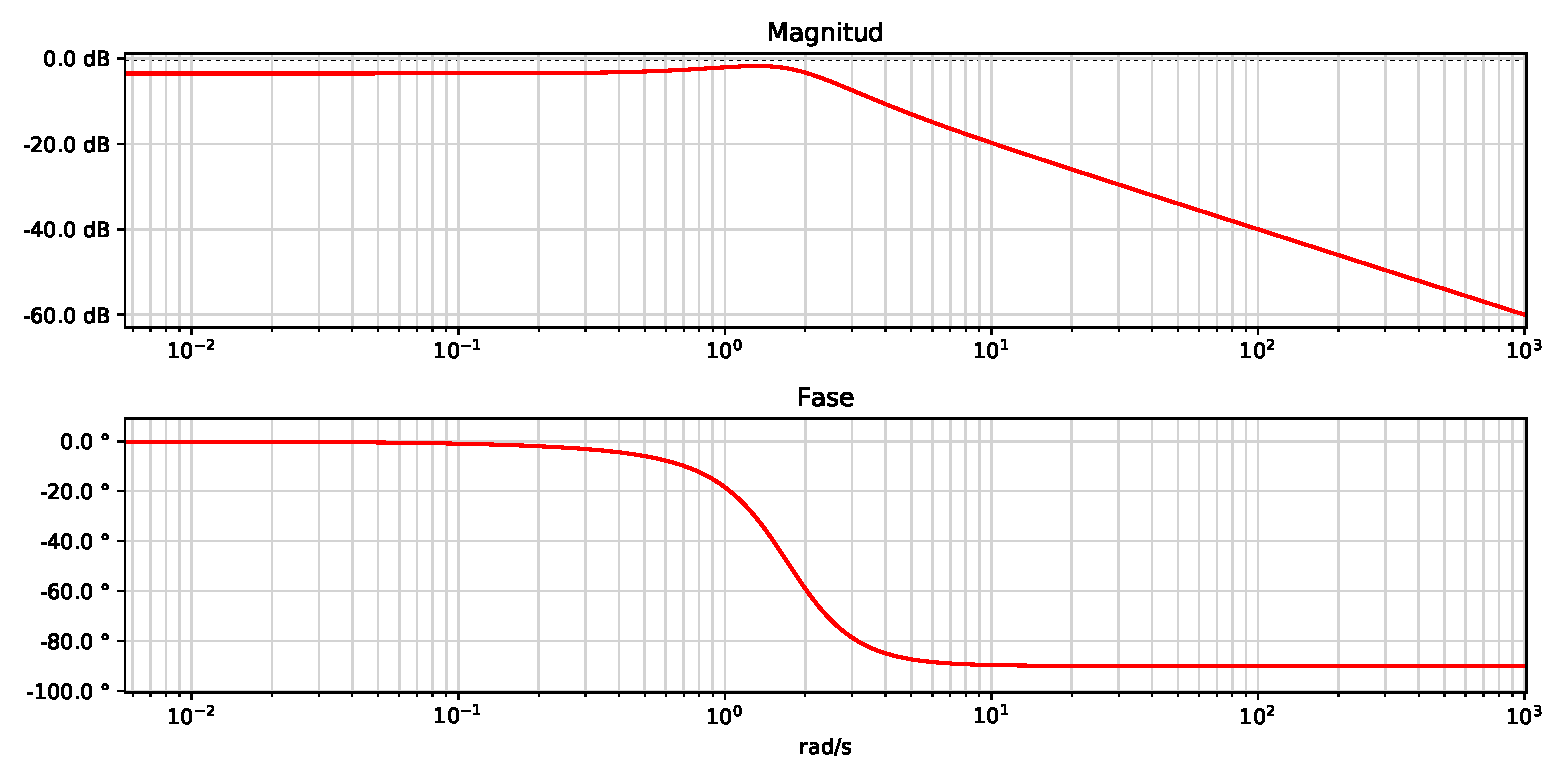
\includegraphics[width=\textwidth]{bodeG1.pdf}
                    \caption[Ejemplo 1 margenes de ganancia y fase]{\textbf{Margenes de ganancia y fase de $G_1(s)$}. En el diagrama se puede observar que no existe cruce por $0dB$ en magnitud o cruce por $-180^\circ$ en fase, por tanto, el sistema es estable y acepta incrementos teoricos de ganancia infinitos . Fuente: Elaboración propia.}
                    \label{fig:bodeG1}
                \end{figure}

                \begin{figure}[htb]
                    \centering
                    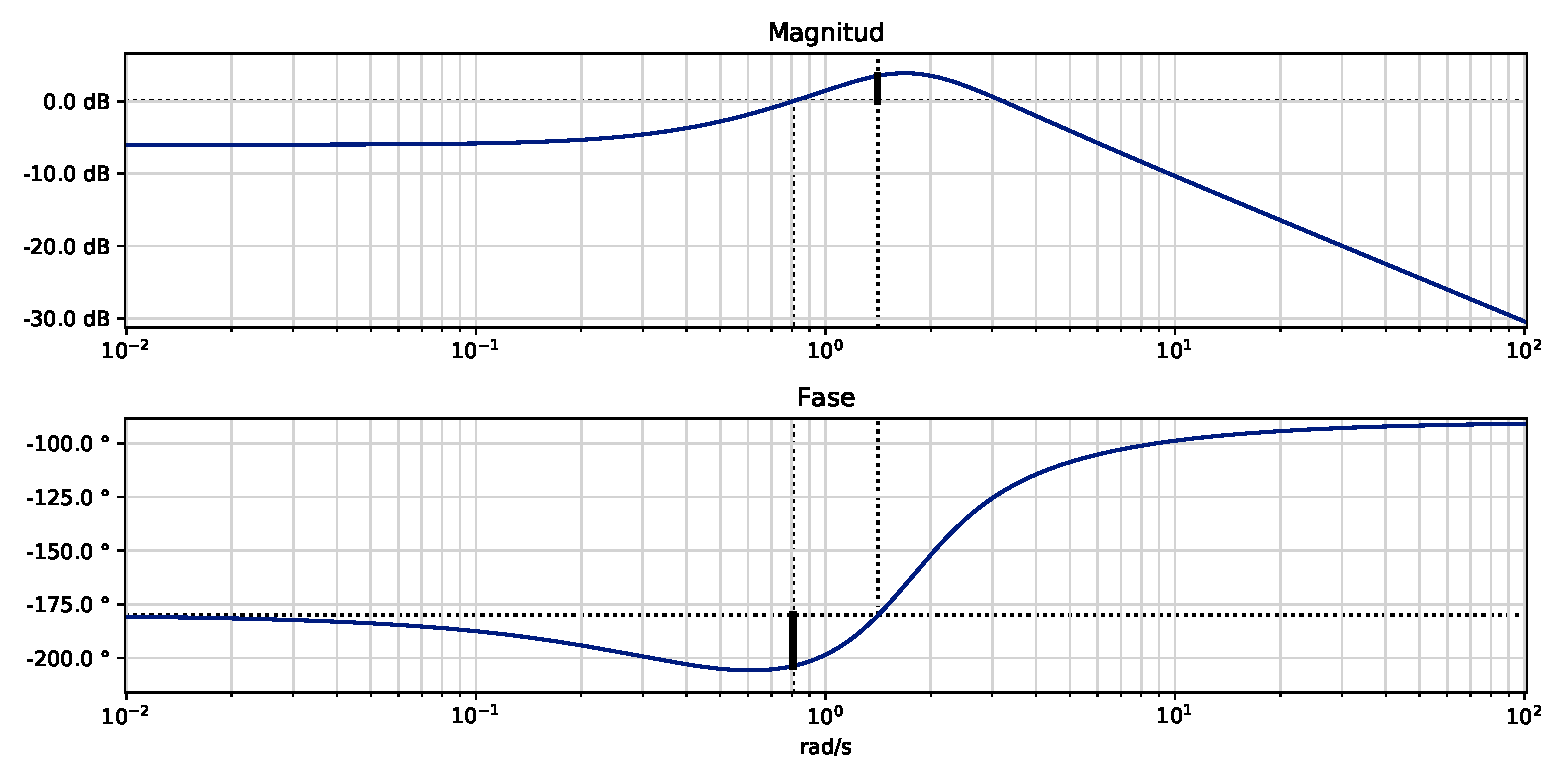
\includegraphics[width=\textwidth]{bodeG2.pdf}
                    \caption[Ejemplo 2 margenes de ganancia y fase]{\textbf{Margenes de ganancia y fase de $G_2(s)$}. El sistema $G_2(s)$ es de fase no minima, por tanto, la interpretacion del margen de ganancia y de fase no es tan simple. En la figura se observar que el margen de ganancia es negativo y aun asi, sabemos por su analisis con diagrama de Nyquist que es estable en lazo cerrado. Fuente: Elaboración propia.} 
                    \label{fig:bodeG2}
                \end{figure}
            
            \paragraph{Diagrama de Nichols}
                
                El diagrama de Nichols es una grafica del sistema en lazo abierto de tipo magnitud vs fase, en el diagrama se pueden ubicar los margenes de ganancia y fase, para ayudar en el diseño de controladores se suele superponer una rejilla guia de valores de magnitud y angulo constantes, esta rejilla lleva el nombre de carta de Nichols o abaco de Nichols. En el diagrama de nichols el punto critico $-1 + j0$ se convierte en $(0dB, -180^\circ)$

                \clearpage

        \subsubsection{Controlador PID}

            El controlador será el elemento dentro del sistema de control que se encargará de llevar al proceso a un valor de referencia deseado, existen varios esquemas de control para el control de procesos, cada uno con sus ventajas y desventajas, el más común es un sistema en lazo cerrado con controlador, este se puede observar en la \cref{fig:esquemaPID}.

            \begin{figure}[htb]
                \centering
                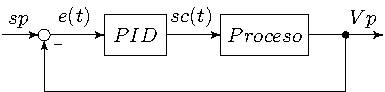
\includegraphics[width=\textwidth]{esquemaPID.pdf}
                \caption[Ejemplo de un sistema en lazo cerrado con controlador]{\textbf{Sistema en lazo cerrado con controlador}. El controlador recibe la señal de error y genera una señal de control $sc(t)$. Fuente: Elaboración propia.} 
                \label{fig:esquemaPID}
            \end{figure}

            En este esquema se observa que el controlador recibe la señal de error producto de tomar la diferencia entre el setpoint y la variable del proceso, este error es utilizado por el controlador para generar una señal de control $sc(t)$. El controlador más usado en la industria es el controlador PID, así lo afirma \textcite{kuo1996sistemas}: \enquote{[...] uno de los controladores más ampliamente empleados es el controlador PID [...] donde las letras son las iniciales de proporcional, integral y derivativo}(p.$\,$671). La ecuación que define a un PID en el dominio del tiempo es la siguiente:

            \begin{equation}\label{eq:pidtiempo}
                sc(t) = K_{p}e(t)+  K_{i}\int_{0}^{t} e(\tau) d\tau + K_{d} \frac{d}{dt}e(t)
            \end{equation}
            
            \noindent y su forma en función de transferencia:
            
            \begin{equation}\label{eq:pidcompleja}
                G_{c}(s) = \frac{sc(s)}{e(s)} = \frac{K_{d}s^{2} + K_{p}s +  K_{i}}{s}
            \end{equation}
            
            El controlador PID tambien puede ser representado de forma discreta, la componente proporcional sigue siendo una constante, la componente integral se puede representar como la sumatoria de todas las muestras multiplicadas por el periodo de muestreo y finalmente la derivada se puede aproximar como una diferencia finita regresiva:

            \begin{equation}\label{eq:pidcdiscreto}
                sc(k) = K_{p}e(k)+  K_{i}T\left[\sum_{i=0}^{k-1} e(i) + e(k)\right] + K_{d} \frac{e(k)- e(k-1)}{T}
            \end{equation}

            En el dominio Z, la componente proporcional se mantiene como constante, la componente integral puede ser aproximada con varios metodos numericos para el calculo de area como la integracion trapezoidal \Parencite{kuo1996sistemas}, o lo que es lo mismo, el metodo de Tustin, para el caso de la derivda se parte de su aproximacion como diferencia finita regresiva y se le aplica la transformada Z.

            \begin{equation}\label{eq:pidenZ}
                G_{c}(z) = K_{p} + \frac{K_{i}T}{2}\left(\frac{z+1}{z-1}\right) + K_{d} \frac{z-1}{Tz}
            \end{equation}

            \paragraph{Componente proporcional}

				La componente proporcional se obtiene de multiplicar la señal de error por la ganancia proporcional, lo cual provoca que la señal de control sea proporcional a la señal de error con una relación igual a la ganancia proporcional, si el controlador solo constase de componente proporcional el error en estado estable nunca se eliminaría, dicho de otro modo, el error podría ser muy bajo, pero jamás cero. \enquote{Este error se denomina la desviación permanente u \enquote{offset}. El mismo disminuye si se aumenta el valor de K}\Parencite[p.$\,$54]{nelson1999fundamentos}.

			\paragraph{Componente integral}

				La componente integral viene dada por la sumatoria de la señal del error en el tiempo multiplicada por la ganancia integral, por tanto, se obtiene una acumulación en un periodo determinado, lo anterior implica que mientras exista error, la componente integral seguirá aumentando o disminuyendo dependiendo del signo de la señal de error hasta que el error sea cero, la componente integral se suma con la componente proporcional formando una única señal de control.

				Debido a que la componente integral depende del tiempo, es posible corregir desviaciones de la variable controlada generadas por perturbaciones externas. Por otro lado, debido a que eventualmente se conseguirá que el error sea igual a cero la componente proporcional no hará ningún aporte al sistema, y la señal de control pasará a ser totalmente generada por la componente integral hasta que exista un cambio en el setpoint o una alteración en la variable medida.

			\paragraph{Componente derivativa}

				La componente derivativa viene dada por el ritmo de cambio de la señal de error multiplicado por la ganancia derivativa, por tanto, cuando el error permanece constante la componente derivativa es igual a cero, la componente derivativa será tan grande como la velocidad con la que cambie el error, lo cual ayuda a evitar que se generen sobre pasos en la variable medida respecto a la variable de referencia.
				
				La componente derivativa es muy sensible al ruido, por tanto, se debe utilizar solo cuando se requiera un cierto grado de anticipación y no exista ruido \Parencite{smith1985principles}. Es recomendable utilizar filtros en orden de disminuir el posible ruido, a su vez, cuando el proceso a controlar es de respuesta rápida se recomienda no agregar componente derivativa o que su ganancia sea muy pequeña. Tomando en cuenta lo anterior, se debe mencionar que la componente derivativa tal como se observa en las ecuaciones \cref{eq:pidtiempo} y \cref{eq:pidcompleja} no es implementable al ser no causal, por tanto, la derivada puede ser implementada utilizando una aproximacion. \blockquote[{\cite[p.220]{aastrom2002control}}]{La aproximacion actua como una derivada para las componentes de la señal de baja frecuencia. La ganancia, sin embargo, esta limitada a $KN$. Esto significa que las medidas de ruido de alta frecuencia son amplificados cuando mucho por un factor $KN$.} La funcion de transferencia de la componente derivativa aproximada es la siguiente:

                \begin{equation}\label{eq:Daproximacion}
                    D = K_d \frac{N s}{s + N}
                \end{equation}

        \subsubsection{Entonación por método de Ziegler-Nichols en lazo abierto}
			
            El método de Ziegler-Nichols en lazo abierto requiere primero aproximar el modelo del proceso como una función de transferencia de primer orden con tiempo muerto.
            
            \begin{equation}\label{eq:firstorderProcess}
                G(s) = \frac{K}{\tau s + 1} e^{-\alpha s}
            \end{equation}
            
            Los parámetros correspondientes pueden ser obtenidos realizando una prueba al escalón y extrayendo los datos correspondientes de la gráfica de la respuesta, un ejemplo se puede observar en la \cref{fig:ZNtest}. Acá se observa: (a) $t_{0}$ que corresponde al inicio del escalón, (b) $t_{1}$ inicio de la respuesta por parte del proceso al escalón, (c) $t_{2}$ cuando el proceso alcanza el 63\% del cambio total, (d) $\Delta y$ cambio total del proceso ante el escalón y (e) $\Delta u$ magnitud de cambio de la entrada. Los parámetros para aproximar el proceso a un modelo de primer orden con tiempo muerto se calculan como sigue:
            
            \begin{align}\label{eq:parametros}
                K &= \frac{\Delta y}{\Delta u}\\
                \tau &= t_{2} - t_{1}\\
                \alpha &= t_{1} - t_{0}
            \end{align}
            
            \begin{figure}[htb]
                \centering
                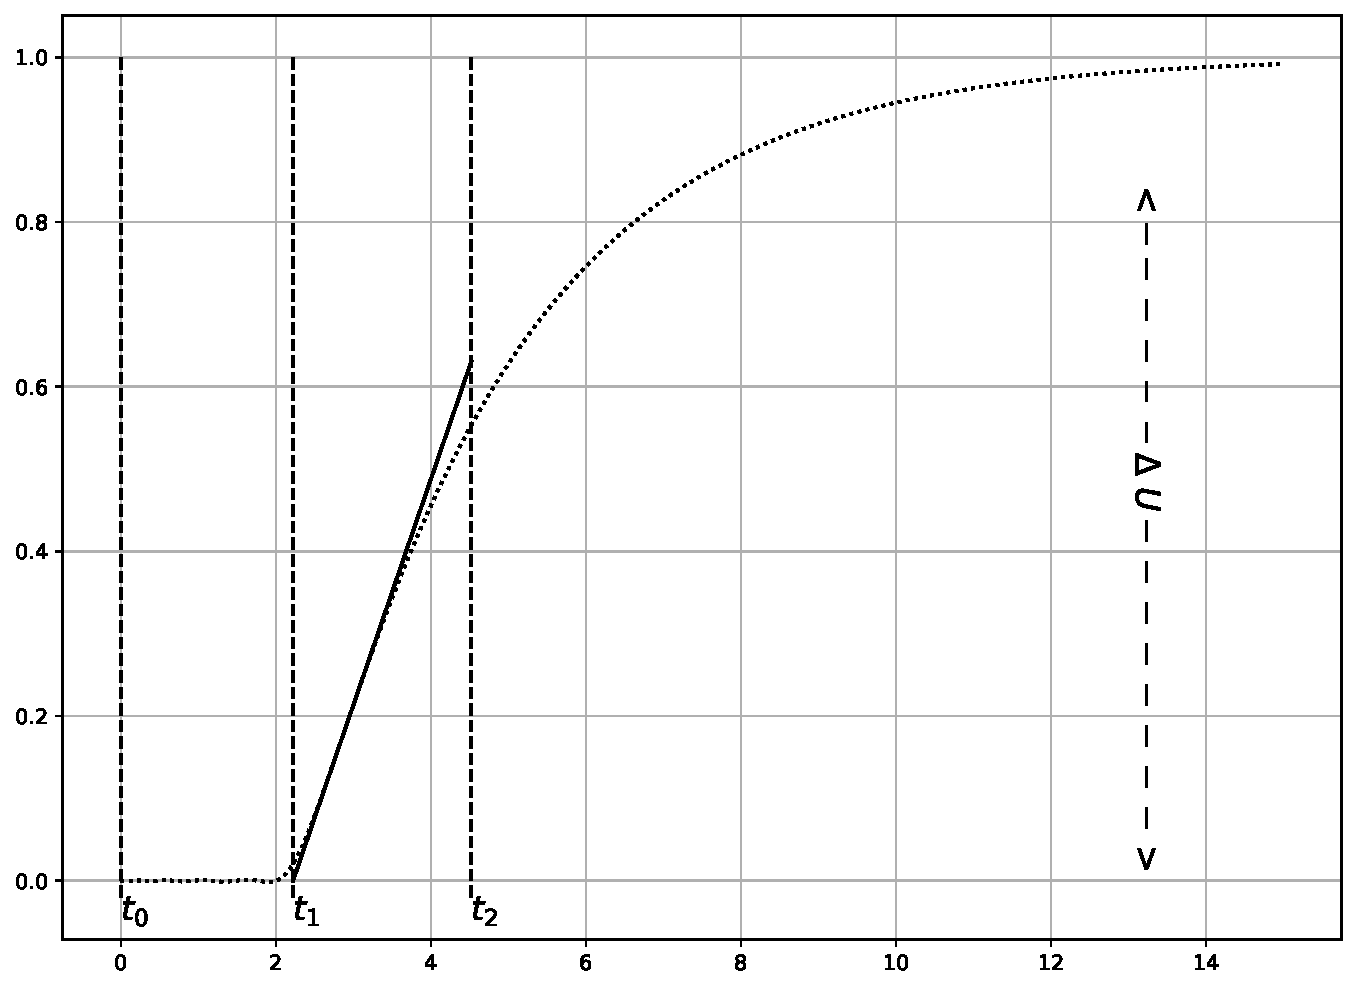
\includegraphics[width=0.85\textwidth]{ZieglerN.pdf}
                \caption[Modelado por curva de reacción]{\textbf{Modelado por curva de reacción.} Para realizar este modelado se estudia la respuesta del sistema ante la entrada de la función de heaviside u(t), también llamada función escalón unitario, el modelo obtenido a través de este método es una aproximación del sistema. Fuente: Elaboración propia.} 
                \label{fig:ZNtest}
            \end{figure}
            
            Con los parametros del modelo de primer orden se puede obtener la entonación de un controlador P, PI o PID. Las ganancias $K_{p}$, $K_{i}$ y $K_{d}$ se pueden obtener sustituyendo los mencionados parametros en la \cref{tab:ZiglerNichols} correspondiente a la regla de entonación de Ziegler-Nichols. \textcite{ogata2003ingenieria} comenta que: \enquote{Las reglas de sintonía de Ziegler-Nichols [...] se han usado ampliamente para sintonizar controladores PID en sistemas de control de procesos en los que no se conoce con precisión la dinámica de la planta}(p.$\,$572).
            
            \begin{table}[htb]
                \centering
                \begin{threeparttable}
                    \renewcommand{\arraystretch}{1.5} 	% Separacion de las filas
                    %\setlength{\tabcolsep}{6pt}			% Separacion de columnas
                    \caption[Regla de entonación de Zigler-Nichols]{Regla de entonación de Zigler-Nichols}
                    \begin{tabular*}{\textwidth}{c @{\extracolsep{\fill}}ccc}
                        \toprule
                        Tipo de controlador & $K_{p}$                               &              $T_{i}$              &         $T_{d}$          \\ \midrule
                                    P          & $\displaystyle\frac{\tau}{\alpha}$    &       $\displaystyle\infty$       &            0             \\[20pt]
                                PI          & $0.9\displaystyle\frac{\tau}{\alpha}$ & $\displaystyle\frac{\alpha}{0.3}$ &            0             \\[20pt]
                                PID         & $1.2\displaystyle\frac{\tau}{\alpha}$ &      $2\displaystyle\alpha$       & $0.5\displaystyle\alpha$ \\ \bottomrule
                    \end{tabular*}
                    \label{tab:ZiglerNichols}
                    \begin{tablenotes}[flushleft]
                        \item {\footnotesize \textbf{Nota.} Los valores de $K_{i}$ y $K_{d}$ se pueden obtener de la siguiente forma: $K_{i} = K_{p}/T_{i}$ ; $K_{d} = K_{p}T_{d}$. Fuente: \textcite{ogata2003ingenieria}.}
                    \end{tablenotes}
                \end{threeparttable}
            \end{table}
            
            Adicionalmente existen otras reglas para la entonacion automatica de los controladore PID, como el metodo de Cohen-Coon, al igual que Ziegler-Nichols, requiere de los parametros del proceso en su aproximacion como proceso de primer orden para ser sustituidos en la \cref{tab:CohenCoon} y obtener las ganancias respectivas.

            \clearpage
            
            \begin{table}[htb]
                \centering
                \begin{threeparttable}
                    \renewcommand{\arraystretch}{1.5} 	% Separacion de las filas
                    %\setlength{\tabcolsep}{6pt}			% Separacion de columnas
                    \caption[Regla de entonación de Cohen-Coon]{Regla de entonación de Cohen-Coon}
                    \begin{tabular*}{\textwidth}{c @{\extracolsep{\fill}}ccc}
                        \toprule
                        Tipo de controlador & $K_{p}$                               &              $T_{i}$              &         $T_{d}$          \\ \midrule \renewcommand{\arraystretch}{3.5}
                                    P          & $\displaystyle\frac{1}{K}\left(\displaystyle\frac{\tau}{\alpha}\right)\left[1 + \displaystyle\frac{1}{3}\left(\displaystyle\frac{\alpha}{\tau} \right) \right]$    &       $\displaystyle\infty$       &            0             \\[25pt]
                                PI          & $\displaystyle\frac{1}{K}\left(\displaystyle\frac{\tau}{\alpha}\right)\left[0.9 + \displaystyle\frac{1}{12}\left(\displaystyle\frac{\alpha}{\tau} \right) \right]$ & $\alpha\left[ \displaystyle\frac{30 + 3\left(\displaystyle\frac{\alpha}{\tau} \right) }{9 + 20\left(\displaystyle\frac{\alpha}{\tau} \right) } \right]$ &            0             \\[25pt]
                                PD & $\displaystyle\frac{1}{K}\left(\displaystyle\frac{\tau}{\alpha}\right)\left[\displaystyle\frac{5}{4} + \displaystyle\frac{1}{6}\left(\displaystyle\frac{\alpha}{\tau} \right) \right]$ & $\displaystyle\infty$ & $\alpha\left[ \displaystyle\frac{6 - 2\left(\displaystyle\frac{\alpha}{\tau} \right) }{22 + 3\left(\displaystyle\frac{\alpha}{\tau} \right) } \right]$ \\[25pt]
                                PID         & $\displaystyle\frac{1}{K}\left(\displaystyle\frac{\tau}{\alpha}\right)\left[\displaystyle\frac{4}{3} + \displaystyle\frac{1}{4}\left(\displaystyle\frac{\alpha}{\tau} \right) \right]$ &      $\alpha\left[ \displaystyle\frac{33 + 6\left(\displaystyle\frac{\alpha}{\tau} \right) }{13 + 8\left(\displaystyle\frac{\alpha}{\tau} \right) } \right]$       & $\alpha\left[ \displaystyle\frac{4}{11 + 2\left(\displaystyle\frac{\alpha}{\tau} \right) } \right]$ \\ \bottomrule
                    \end{tabular*}
                    \label{tab:CohenCoon}
                    \begin{tablenotes}[flushleft]
                        \item {\footnotesize \textbf{Nota.} Los valores de $K_{i}$ y $K_{d}$ se pueden obtener de la siguiente forma: $K_{i} = K_{p}/T_{i}$ ; $K_{d} = K_{p}T_{d}$. Fuente: \textcite{apcoCC}.}
                    \end{tablenotes}
                \end{threeparttable}
            \end{table}

    \subsection{Lógica difusa}
    
        La lógica difusa es una extensión matemática de la lógica convencional en donde se asigna un grado de pertenencia a un hecho entre un valor verdadero y uno falso, \enquote{consiste en que los valores verdaderos (en lógica difusa) o valores de pertenencia (en conjuntos difusos) se indican en un número entre [0.0, 1.0], donde 0.0 representa falsedad total y 1.0 significa verdad absoluta}\Parencite[p.$\,$4]{cruz2010inteligencia}.
        
        La lógica difusa se puede estructurar en tres etapas, la primera etapa consiste en establecer cada una de las variables con etiquetas lingüística que determinen en conjunto el universo de discurso de cada una de ellas, es decir, se crean los conjuntos difusos, en la segunda etapa se definen las reglas de inferencia difusa que determinaran el comportamiento del sistema difuso, y tercera, se obtienen los valores de salida utilizando las reglas de inferencia y realizando el proceso de defuzzificación que consiste en llevar los grados de pertenencia a un valor nítido o real \Parencite{cruz2010inteligencia}. Continuando con la idea, tambien es posible ver la logica como cuatro procedimientos a realizar en secuencia, las cuales son: fuzzificación, inferencia, agregacion y defuzzificación.
        
        \subsubsection{Conjuntos difusos}
            
            Un conjunto difuso está compuesto de funciones de membresía, dichas funciones de membresía representan valores para asignar el grado de pertenencia de una variable a un estado en particular y son identificados con etiquetas lingüísticas descriptivas, como alto, caliente, bajo, negativo, entre otras. En la \cref{fig:FuzzySet} se puede observar un ejemplo de conjunto difuso.
            
            \begin{figure}[htb]
                \centering
                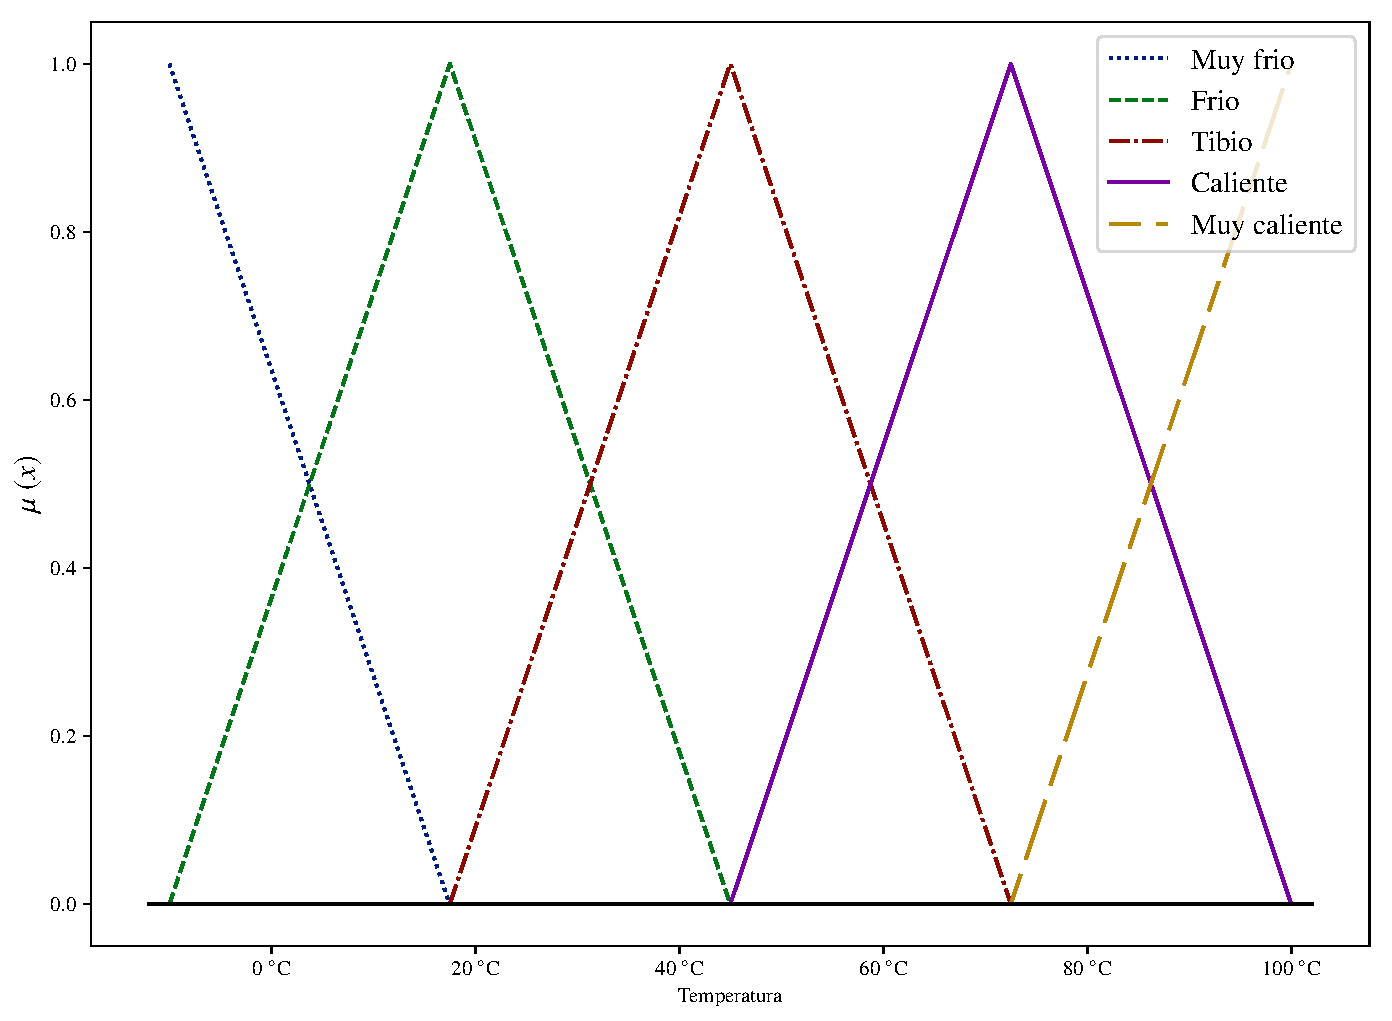
\includegraphics[width=0.6\textwidth]{FuzzySet.pdf}
                \caption[Ejemplo de un conjunto difuso]{\textbf{Ejemplo de un conjunto difuso}. Este conjunto difuso corresponde a una variable de temperatura que va desde -10\textdegree C hasta 100\textdegree C. Fuente: Elaboración propia.} 
                \label{fig:FuzzySet}
            \end{figure}
            
            Las funciones de membresía pueden tomar varias formas y rangos en orden de poder representar de mejor forma los grados de pertenencia de la variable a una etiqueta en particular, sin embargo, las formas triangulares suelen ser las menos pesadas en memoria y en poder de cómputo \Parencite{riid2003transparent}. La cantidad de etiquetas que se pueden asignar a un conjunto difuso es ilimitada, pero se debe tener en cuenta el nivel de complejidad que se genera a medida que se incrementa su número. A continuacion se muestran algunas formas que pueden tomar las funciones de membresia:

            \paragraph{Funcion de membresia: triangular o trimf}$\quad$
            
            \begin{equation*}\label{eq:trimf}
                \mu_n(x) = \left\{
                    \begin{aligned}
                        &\quad 0  &\quad &Si \quad & x &\leq a\\
                        &\frac{x - a}{b - a}  &\quad &Si \quad &  a \le &x \leq b \\
                        &\frac{c - x}{c - b}  &\quad &Si \quad & b \le &x \leq c \\
                        &\quad 0  &\quad &Si \quad&  x &\geq c
                    \end{aligned}\right.
                    \qquad
                    \raisebox{-15mm}{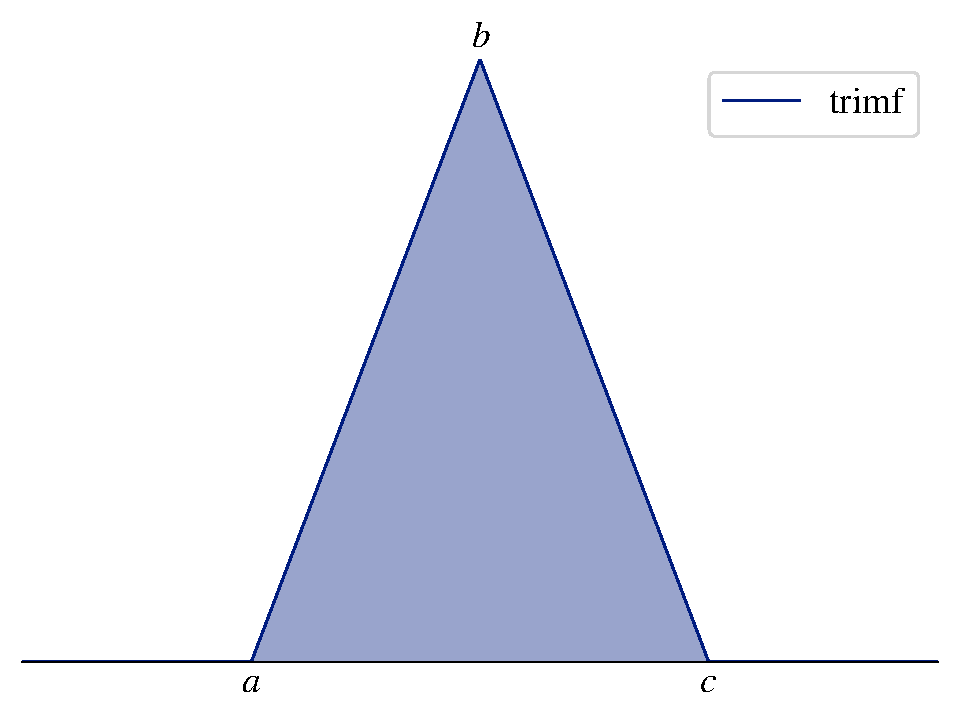
\includegraphics[width=0.28\linewidth]{trimf.pdf}}
            \end{equation*}
            
            \paragraph{Funcion de membresia: trapezoidal o trapmf}$\quad$
            
                \begin{equation*}\label{eq:trapmf}
                    \mu_n(x) = \left\{
                        \begin{aligned}
                            &\quad 0  &\quad &Si \quad &  x &\leq a\\
                            &\frac{x - a}{b - a}  &\quad &Si \quad &  a \le &x \leq b \\
                            &\quad 1 &\quad &Si \quad &  b \le &x \leq c \\
                            &\frac{d - x}{d - c}  &\quad &Si \quad & c \le &x \leq d \\
                            &\quad 0  &\quad &Si \quad & x &\geq d
                        \end{aligned}\right.
                        \qquad
                        \raisebox{-15mm}{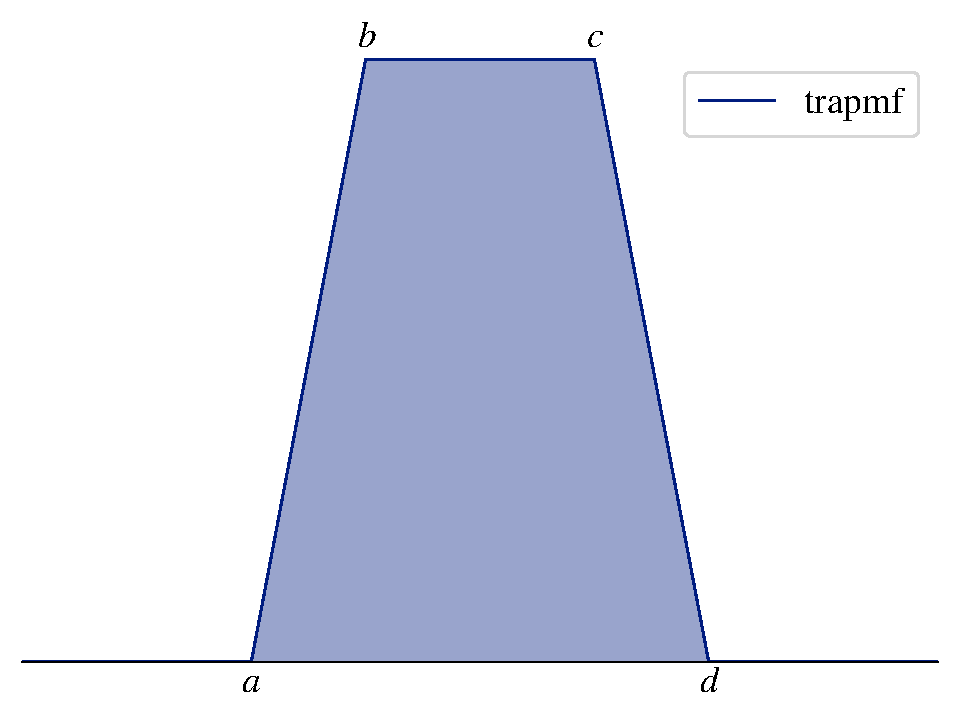
\includegraphics[width=0.28\linewidth]{trapmf.pdf}}
                \end{equation*}

            \paragraph{Funcion de membresia: gaussiana o gaussmf}$\quad$
                
                \begin{equation*}\label{eq:gaussmf}
                    \mu_n(x) = e^{-\frac{(x-m)^2}{2\sigma^2}}
                        \qquad \qquad
                        \raisebox{-15mm}{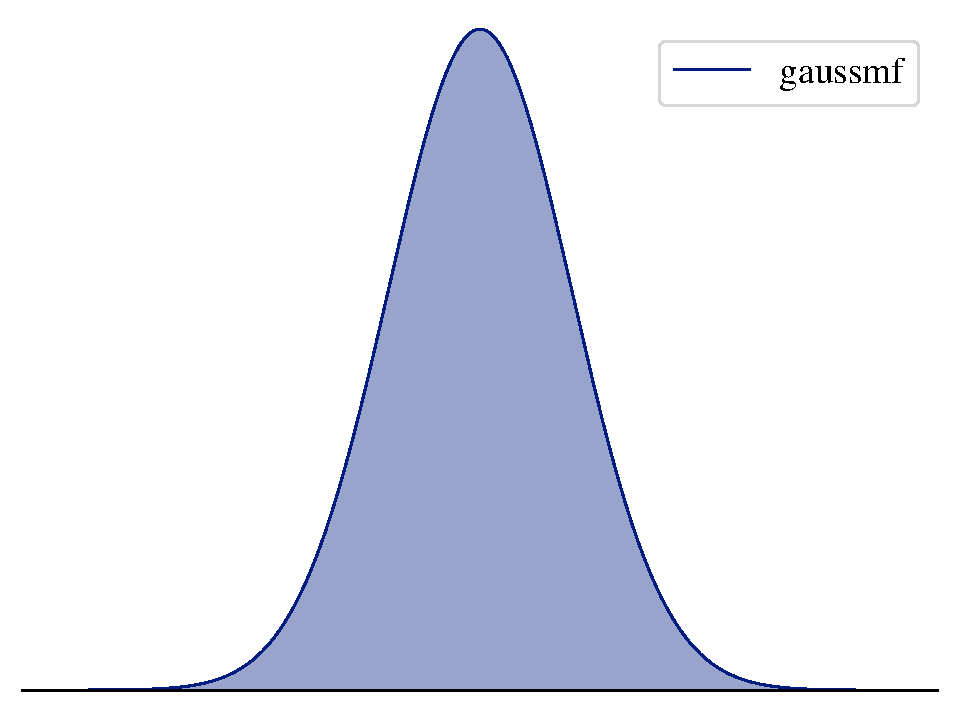
\includegraphics[width=0.28\linewidth]{gaussmf.pdf}}
                \end{equation*}
                
            \paragraph{Funcion de membresia: S o smf}$\quad$
                
                \begin{equation*}\label{eq:smf}
                    \mu_n(x) = \left\{
                        \begin{aligned}
                            &\quad 0  &\quad &Si \quad & x &\leq a\\
                            &2\left(\frac{x - a}{b - a}\right)^2  &\quad &Si \quad &  a \leq &x \leq \frac{a+b}{2} \\
                            &1 - 2\left(\frac{x - b}{b - a}\right)^2  &\quad &Si \quad & \frac{a+b}{2} \leq &x \leq b \\
                            &\quad 1  &\quad &Si \quad & x &\geq b
                        \end{aligned}\right.
                        \qquad
                        \raisebox{-15mm}{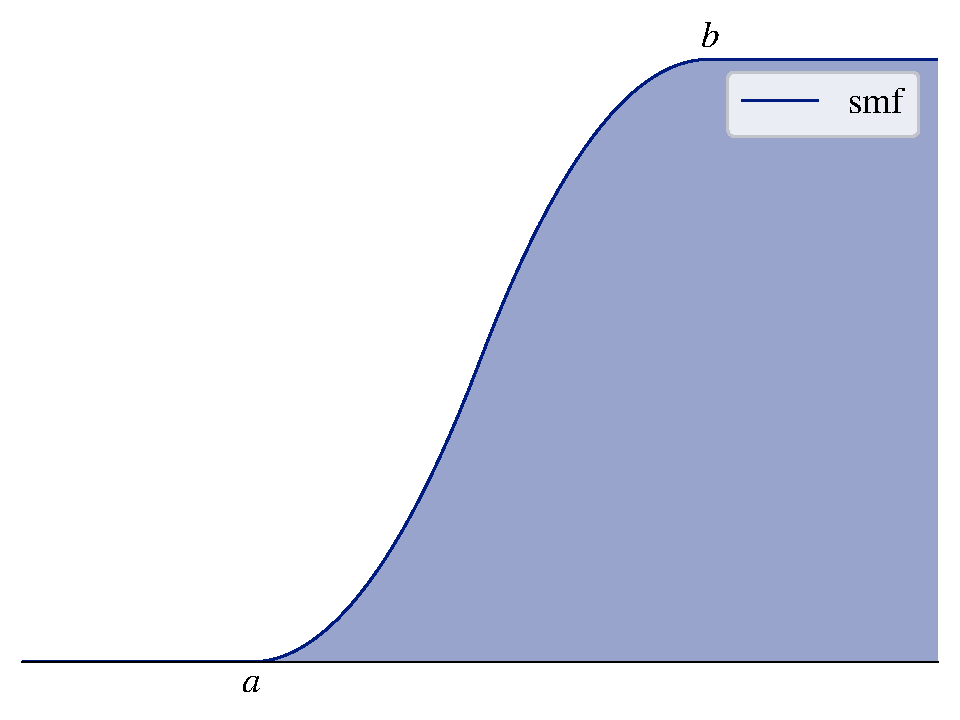
\includegraphics[width=0.28\linewidth]{smf.pdf}}
                \end{equation*}
            
            \paragraph{Funcion de membresia: Z o zmf}$\quad$
                
                \begin{equation*}\label{eq:zmf}
                    \mu_n(x) = \left\{
                        \begin{aligned}
                            &\quad 1  &\quad &Si \quad & x &\leq a\\
                            &1 - 2\left(\frac{x - a}{b - a}\right)^2  &\quad &Si \quad &  a \leq &x \leq \frac{a+b}{2} \\
                            &2\left(\frac{x - b}{b - a}\right)^2  &\quad &Si \quad & \frac{a+b}{2} \leq &x \leq b \\
                            &\quad 0  &\quad &Si \quad & x &\geq b
                        \end{aligned}\right.
                        \qquad
                        \raisebox{-15mm}{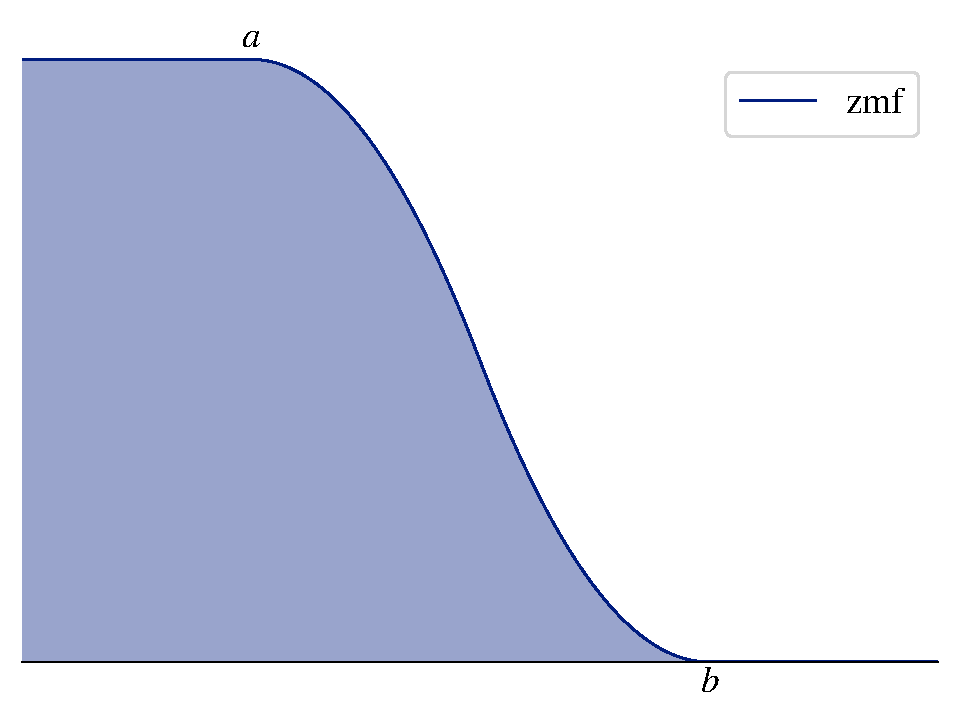
\includegraphics[width=0.28\linewidth]{zmf.pdf}}
                \end{equation*}

            \paragraph{Funcion de membresia: sigmoidal o sigmf}$\quad$
                
                \begin{equation*}\label{eq:sigmf}
                    \mu_n(x) = \frac{1}{1+e^{-c(x-b)}}
                        \qquad \qquad
                        \raisebox{-15mm}{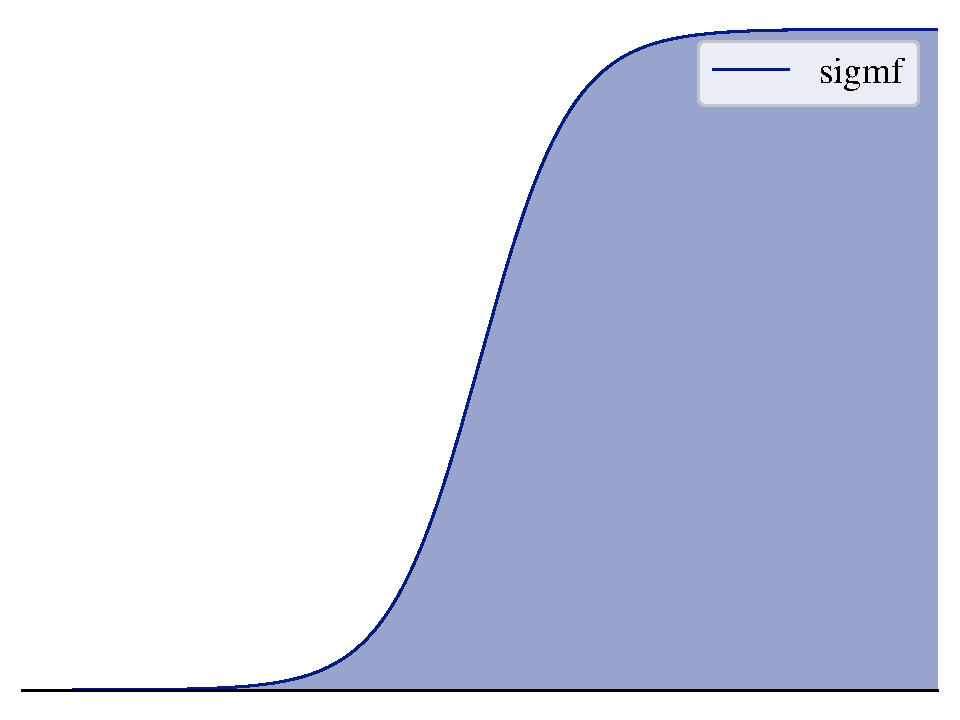
\includegraphics[width=0.28\linewidth]{sigmf.pdf}}
                \end{equation*}
               
            \paragraph{Funcion de membresia: campana generalizada o gbellmf}$\quad$
                
                \begin{equation*}\label{eq:gbellmf}
                    \mu_n(x) = \frac{1}{1+ \left|\frac{x - c}{a}\right|^{2b}}
                        \qquad \qquad
                        \raisebox{-15mm}{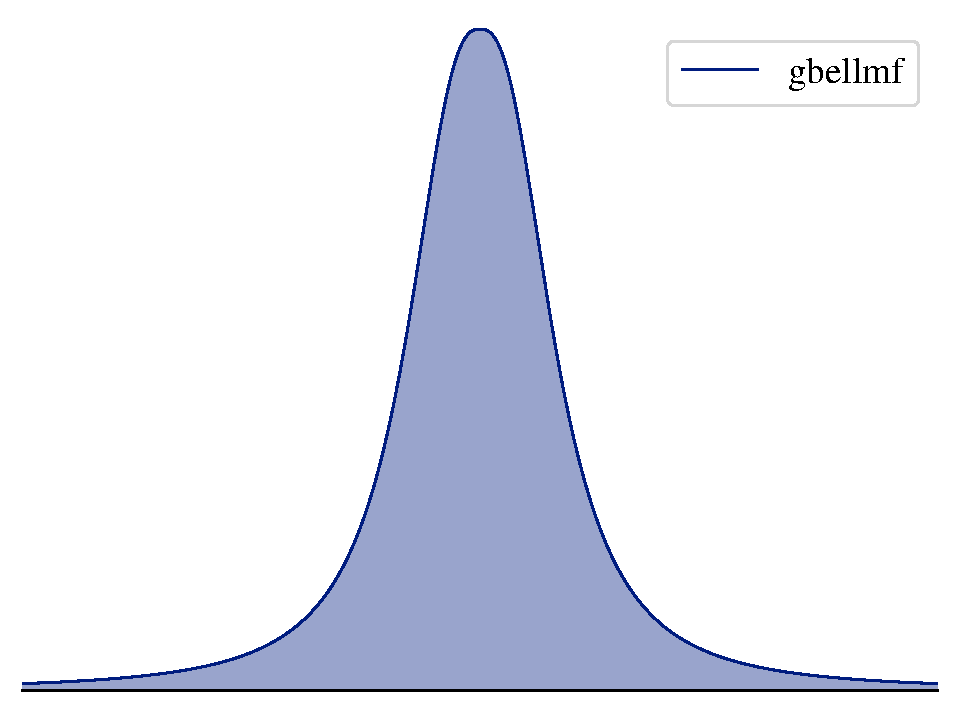
\includegraphics[width=0.28\linewidth]{gbellmf.pdf}}
                \end{equation*}

            Existen otras funciones de membresian que utilizan como base las anteriores mostradas, estas son:

            \begin{itemize}[leftmargin=\parindent]
                \item gauss2mf: Combinacion de dos funciones gaussianas.
                \item dsigmf: Valor absoluto de la diferencia de dos funciones sigmoidales.
                \item psigmf: Producto de dos funciones sigmoidales.
                \item pimf: Producto de una smf y una zmf.
            \end{itemize}
        
        \subsubsection{Reglas de inferencia}
            
            Las reglas de inferencia, al igual que en la lógica convencional, se encargan de realizar una conexión entre los antecedentes y los consecuentes con el fin de obtener una salida, en este caso, entre los conjuntos difusos de entrada y salida, la salida puede ser un conjunto difuso o una función matemática. Como sugiere \textcite{cruz2010inteligencia}, las reglas pueden formularse de dos formas denominadas modus ponens y modus tollens. Modus ponens utiliza los antecedentes para obtener el consecuente, por otro lado, el modus tollens utiliza los consecuentes recíprocos para obtener el antecedente.
                        
            Para realizar el proceso de inferencia se debe haber pasado primero por la fuzzificacion, la cual implica tomar los valores de entrada y obtener sus valores de pertenencia para cada funcion de membresia, luego, se aplican las normas triangulares (T-Normas) para el caso de logica AND o las conormas triangulares (T-Conormas) para logica OR, sus formas de aplicacion mas comunes suelen ser el minimo de los valores de pertenencia para las T-Normas y el maximo de los valores de pertenencia para las T-Conormas, de este modo, se obtienen las operaciones de interseccion y union respectivamente, a este proceso tambien se le conoce como conjuncion de premisas para las T-Normas y disyuncion de premisas para las T-Conormas.
            
            Luego de este proceso se debe seguir con la operacion de implicacion, usualmente se realiza y se prefiere con la conjuncion (T-Normas), esta viene definida por:

            \begin{equation}\label{eq:implicacion}
                F_r(y) = \tau_r \cap \gamma_r
            \end{equation}

            Donde $\tau_r$ es la salida del proceso de conjuncion/disyuncion de premisas y $\gamma_r$ es la salida de la funcion de membresia asociada con la $r$-esima regla \Parencite{riid2003transparent}. Una vez realizado este proceso, se puede procedar a realizar la agregacion.
        
        \subsubsection{Agregacion}

            El proceso de agregacion se realiza luego de haber pasado por la fuzzificacion, conjuncion/disyuncion de premisas y la implicacion, a todos los resultados obtenidos se les aplica un operador OR por medio de una T-Conorma, de este modo, se obtiene un conjunto difuso que representa a la salida . Todo el proceso hasta este punto puede ser descrito asumiendo conjuncion de premisas por la siguiente formula:

            \begin{equation}\label{eq:implicacion}
                F(y) = \bigcup_{r=1}^{R}\left(\left(\bigcap_{i=1}^{N}\tau_{ir} \right) \cap \gamma_r\right)
            \end{equation}
            
            \noindent sin embargo, esta salida aun no es apta para ser interpretada, por tanto, debe pasar primero por un proceso de defuzzificación en orden de llevar el conjunto difuso de salida a un valor nitido.

        \subsubsection{Defuzzificación}

            En esta última etapa también llamada desdifusificación, se obtienen los valores reales de salida, \textcite{cruz2010inteligencia} lo describe como el \enquote{[...] mapeo a escala que convierte el rango de valores de las variables de salida a sus universos de discurso correspondientes. La desdifusificación es la herramienta para obtener la acción de control nítida a partir de una acción de control difusa} (p.$\,$73). Este proceso es matemáticamente costoso y existen distintos métodos para realizarlo, el más común es el método de centro de área.
            
            \paragraph{Método de centro de área}

                Este método se utiliza para realizar la defuzzificación y obtener las salidas nítidas, consiste en cortar las funciones de membresía $\mu_{n}(x)$ con los valores de entrada $x$ para determinar un área. El área inferior será la que se tome en cuenta para realizar el cálculo, el método de centro de área se puede representar de modo general en su forma discreta de la siguiente forma:
                
                \begin{equation}\label{eq:Centroide}
                    Salida = \frac{\displaystyle\sum\limits_{x=a}^{b}\mu_{n}(x)\cdot x}{\displaystyle\sum\limits_{x=a}^{b}\mu_{n}(x)}
                \end{equation}

            \paragraph{Metodo de bisector de area}
                
                Este metodo ubica un punto en el conjunto difuso de salida y sus valores de pertenencia tal que el area resultante quede dividida en dos partes iguales.

            \paragraph{Metodo de la media del maximo}
                
                Este metodo obtiene una salida a partir de promediar los valores de pertenencia maximos del conjunto difuso de salida.

            \paragraph{Metodo del primero a la izquierda}
                
                Este metodo obtiene una salida a partir de los valores de pertenencia maximos del conjunto difuso de salida, de todos ellos, toma el ubicado mas a la izquierda, o lo que es lo mismo, el menor de ellos.
            
            \paragraph{Metodo del primero a la derecha}
                
                Este metodo obtiene una salida a partir de los valores de pertenencia maximos del conjunto difuso de salida, de todos ellos, toma el ubicado mas a la derecha, o lo que es lo mismo, el mayor de ellos.

        \subsubsection{Sistemas de control difusos}
            
            Un controlador difuso es cualquier tipo de controlador que utilice en su interior alguna forma de lógica difusa, al igual que con los controladores clásicos el esquema de control más común es en lazo cerrado. El controlador difuso a su vez puede contener todo tipo de metodologías de control, de hecho, el uso más común es realizar un controlador P, PI, PD o PID, todos difusos. Para realizar los controladores se puede utilizar la estructura Mamdani, la cual asigna conjuntos difusos para las entradas y para las salidas, por tanto, es necesario el proceso de defuzzificación, comúnmente con el método de centro de área.
            
            No existen métodos analíticos claros para el diseño de controladores difusos, por tanto, se debe realizar bajo la experiencia del diseñador, tomando en cuenta las necesidades de control y las dinámicas del proceso. Lo anterior es debido a que el controlador difuso depende enteramente de la estructura de los conjuntos difusos y de la asignación de las reglas de inferencia \Parencite{cruz2010inteligencia}. Los siguientes esquemas de control fueron tomados de \textcite{cruz2010inteligencia}, \textcite{riid2003transparent}, y \textcite{clavier2017tecnicas}.

            \paragraph{Controlador P difuso}
                
                Un controlador P difuso simple puede ser realizado al tomar como entrada la señal de error y como salida la señal de control. El esquema de control se puede observar en la \cref{fig:pFuzzyTomo}.

                \begin{figure}[htb]
                    \centering
                    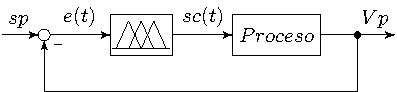
\includegraphics[width=0.6\textwidth]{pFuzzyTomo.pdf}
                    \caption[Esquema de control: P difuso]{\textbf{Esquema de control: P difuso}. Fuente: Elaboración propia.} 
                    \label{fig:pFuzzyTomo}
                \end{figure}

            \paragraph{Controlador PD difuso}
                
                Un controlador PD difuso puede ser realizado al tomar la señal de error y la derivada del error como entradas del controlador y se toma como salida la señal de control. El esquema de control se puede observar en la \cref{fig:pdFuzzyTomo}.

                \begin{figure}[htb]
                    \centering
                    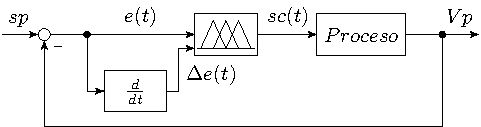
\includegraphics[width=0.7\textwidth]{pdFuzzyTomo.pdf}
                    \caption[Esquema de control: PD difuso]{\textbf{Esquema de control: PD difuso}. Fuente: Elaboración propia.} 
                    \label{fig:pdFuzzyTomo}
                \end{figure}
            
            \paragraph{Controlador PI difuso}
                
                Un controlador PI difuso se puede obtener al agregar un integrador a la salida de un PD difuso, de este modo $sc(t) = e(t) + \Delta e(t)$ se transforma en $sc(t) = \int_0^t e(\tau)d\tau + e(t)$ la cual sera tomada como la señal de control. El esquema de control se puede observar en la \cref{fig:piFuzzyTomo}.

                \begin{figure}[htb]
                    \centering
                    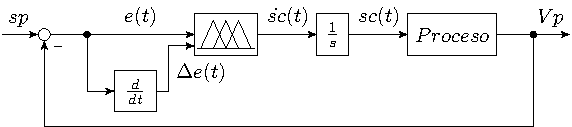
\includegraphics[width=0.7\textwidth]{piFuzzyTomo.pdf}
                    \caption[Esquema de control: PI difuso]{\textbf{Esquema de control: PI difuso}. Fuente: Elaboración propia.} 
                    \label{fig:piFuzzyTomo}
                \end{figure}

            \paragraph{Controlador PID difuso}
                
                Un controlador PD difuso puede ser realizado al tomar la señal de error, la derivada del error y la segunda derivada del error como entradas del controlador, la señal de salida es luego integrada de modo que $sc(t) = e(t) + \Delta e(t) + \Delta^2 e(t)$ se transforma en $sc(t) = \int_0^t e(\tau)d\tau + e(t) + \Delta e(t)$ la cual sera tomada como la señal de control. El esquema de control para un PID difuso completo se puede observar en la \cref{fig:pidFuzzyTomo}.

                \begin{figure}[htb]
                    \centering
                    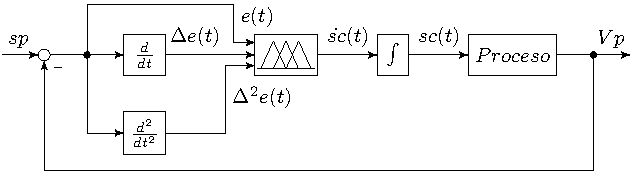
\includegraphics[width=0.8\textwidth]{pidFuzzyTomo.pdf}
                    \caption[Esquema de control: PID difuso]{\textbf{Esquema de control: PID difuso}. Fuente: Elaboración propia.} 
                    \label{fig:pidFuzzyTomo}
                \end{figure}

                Existen otras formas de obtener un PID difuso, una de estas formas es realizando la suma de las salidas de un PD difuso y PI difuso, por otro lado, tambien se puede realizar haciendo uso de componentes no difusos, i.e., sumar la salida de un PD difuso con la integral del error o sumar la salida de un PI difuso con la derivada del error.

            \paragraph{Controlador difuso como programador de ganancias}
                
                El esquema de control difuso con programdor de ganancias consiste en dos controladores, uno difuso y un PID clásico, el controlador difuso se encargará de generar las ganancias del PID de forma dinámica en función de las entradas que reciba, a su vez, el PID será quien gobierne al proceso, por lo cual permite adaptar el controlador PID a los cambios de carga y a los cambios del setpoint. El esquema de control se puede observar en la \cref{fig:GainschedulerTomo}.

                \begin{figure}[htb]
                    \centering
                    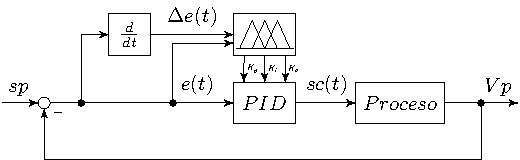
\includegraphics[width=0.8\textwidth]{GainschedulerTomo.pdf}
                    \caption[Esquema de control: Programador de ganancias]{\textbf{Esquema de control: Programador de ganancias}. Fuente: Elaboración propia.} 
                    \label{fig:GainschedulerTomo}
                \end{figure}
            
            \paragraph{Controlador combinado}
                
                Consiste en sumar las salidas de un controlador PID clasico y un controlador difuso, de este modo el controlador PID sera quien gobierne al proceso la mayoria del tiempo, para el caso de un controlador P difuso al generarce un cambio en el setpoint o la carga el controlador difuso procesedera a emitir una salida proporcional y adaptada al cambio. El esquema de control se puede observar en la \cref{fig:pidplusFuzzyTomo}.
            
                \begin{figure}[htb]
                    \centering
                    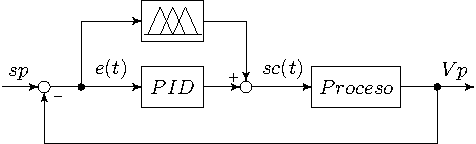
\includegraphics[width=0.8\textwidth]{pidplusFuzzyTomo.pdf}
                    \caption[Esquema de control: PID clasico mas difuso]{\textbf{Esquema de control: PID clasico mas difuso}. Fuente: Elaboración propia.} 
                    \label{fig:pidplusFuzzyTomo}
                \end{figure}

    \subsection{Python}
        
        Python es un lenguaje de programación interpretado y multiparadigma ya que soporta programación orientada a objetos, imperativa y en menor medida funcional. \textcite{guido2017tutorial} afirma que Python es un lenguaje de programación potente que puede aprenderse fácilmente. Cuenta con estructuras de datos eficientes y de alto
        nivel y un enfoque simple pero efectivo a la programación orientada a objetos. La elegante sintaxis de Python y su escritura
        dinámica, junto con su naturaleza interpretada, hacen de éste un lenguaje ideal para scripting y desarrollo rápido de
        aplicaciones en diversas áreas y sobre la mayoría de las plataformas.
        
        Adicionalmente, Python posee bibliotecas externas para realizar cálculos numéricos complejos, también existen bibliotecas para el análisis de sistemas de control y para el diseño de controladores difusos, por otro lado, existen bibliotecas para salidas gráficas con calidad de publicación, gráficas en tiempo real y en 3D.
        
        \subsubsection{Biblioteca NumPy}

            NumPy es una biblioteca para realizar cálculos computacionales científicos y matemáticos, algunas de sus funciones son: cálculo de vectores n-dimensionales, transformada de Fourier, álgebra lineal, entre otras \Parencite{numpy}

        \subsubsection{Biblioteca SciPy}	

            El paquete SciPy es un conjunto de bibliotecas matemáticas, científicas y de ingeniería compuestas por: NumPy, SciPy (biblioteca), SymPy, Matplotlib, IPython y Pandas, la biblioteca SciPy es uno de los núcleos del paquete SciPy. Provee varias rutinas eficientes de uso amigable para el usuario de tipo numérica para realizar integración, interpolación, optimización, álgebra lineal, estadísticas, entre otras \Parencite{scipy}, toda la documentación puede ser conseguida en la página oficial de SciPy.
            
        \subsubsection{Biblioteca Matplotlib}

            Matplotlib es una biblioteca para la graficación 2D que produce figuras con calidad de publicación en varios formatos y a través de múltiples ambientes interactivos. Matplotlib puede ser usado en scripting, consolas de comando, IPython, jupyter notebooks y en aplicaciones web \Parencite{Hunter:2007}. La sintaxis para usar Matplotlib es muy similar al sistema de plots de MATLAB, del mismo modo, configurar parámetros de estilos, fuentes, anchos de línea, entre otros, se realiza de manera similar.

        \subsubsection{Biblioteca de control}

            La biblioteca control de python es un conjunto de clases y funciones que implementan las operaciones más comunes en sistemas de control, además, posee un módulo de compatibilidad para usuarios de MATLAB que emula las funciones y sintaxis de este lenguaje \Parencite{pythoncontrol}. Para crear el modelo de un sistema podemos usar ecuaciones de espacio de estado o funciones de transferencia.

        \subsubsection{Biblioteca Scikit-Fuzzy}
            
            Scikit-Fuzzy es una colección de algoritmos de lógica difusa con la intención de pertenecer al paquete de herramientas científicas SciPy, esta biblioteca permite diseñar y simular controladores difusos con estructura tipo Mamdani \Parencite{warner2016fuzzy}, no posee un modo para realizar lazos de control o compatibilidad con la biblioteca de control de forma directa, de modo que se tendrían que codificar aparte las rutinas que conformen un lazo cerrado de control.

        \subsubsection{Biblioteca PySide2}

            PySide2 es una biblioteca que hace de union entre Qt y Python para la creacion de interfacez de usuario. PySide2 es soportado por linux, Mac OS x, windows, entre otros.
            
        \subsubsection{Biblioteca PyQtGraph}
                
            PyQtGraph es una biblioteca de graficacion especializada en graficas dinamicas y en tiempo real, utiliza de fondo un nucleo Qt, por tanto, requiere el uso de PyQt4, PyQt5, PySide o PySide2.